%%%%%
%%
%% Chalmers University of Technology Master's Thesis Template
%%
%% Jonas Einarsson (2010)
%% Adapted from work by Joel Goop
%%
%% Uses references.bib as Bibtex source
%% Uses elsevier numerical style .bst (change in settings.tex)
%%
%% DON'T FORGET: Change PDF metadata in settings.tex !!
%%
%%%%%
\documentclass[11pt,a4paper,twoside,openright]{report}

% Packages and commands file
\usepackage[utf8]{inputenc}
\usepackage[T1]{fontenc}
\usepackage[english]{babel}
\usepackage{amsmath}
\usepackage{ae}
\usepackage{icomma}
\usepackage{units}
\usepackage{color}
\usepackage{graphicx}
\usepackage{epstopdf}
%\usepackage{subfigure}
\usepackage{bbm}
\usepackage[square, numbers, sort]{natbib}
\usepackage{multirow}
\usepackage{array}
\usepackage[font=footnotesize,format=plain,labelfont=bf,up]{caption}
\usepackage{subfig}
\usepackage{geometry}
\usepackage{fancyhdr}
\usepackage{fncychap}
\usepackage[hyphens]{url}
\usepackage[breaklinks,pdfpagelabels=false]{hyperref}
\usepackage{lettrine}
\usepackage{eso-pic}

\newcommand{\rd}{\ensuremath{\mathrm{d}}}
\newcommand{\id}{\ensuremath{\,\rd}}
\newcommand{\degC}{\ensuremath{\,\unit{^\circ C}}}

% Fancyheader shortcuts
\newcommand{\setdefaulthdr}{%
\fancyhead[L]{\slshape \rightmark}%
\fancyhead[R]{ }%
\fancyfoot[C]{\thepage}%
}
\newcommand{\setspecialhdr}{%
\fancyhead[L]{ }%
\fancyhead[R]{\slshape \leftmark}%
\fancyfoot[C]{\thepage}%
}

\newcommand{\mail}[1]{\href{mailto:#1}{\nolinkurl{#1}}}
\newcommand{\backgroundpic}[3]{%
	\put(#1,#2){
		\parbox[b][\paperheight]{\paperwidth}{%
			\centering
			\includegraphics[width=\paperwidth,height=\paperheight,keepaspectratio]{#3}
			\vfill
}}}


%\usepackage{subcaption}


% Settings (Metadata)
% References, choose bst-file
\bibliographystyle{elsart-num}

% PDF Metadata and link styles
\hypersetup{
		pdftitle={Modelling of electrokinetic flow using the lattice-Boltzmann method},%
		pdfauthor={Andreas B\"{u}lling},%
    colorlinks=true,%
    citecolor=black,%
    filecolor=black,%
    linkcolor=black,%
    urlcolor=black
}

% Dropping initial letter color
\renewcommand{\LettrineFontHook}{\color[gray]{0.5}}

% Chapter headings style (fncychap)
\makeatletter
\ChNumVar{} % sets the style for digit
\ChTitleVar{\Huge\bfseries\centering} % sets the style for title
\ChRuleWidth{4pt} % Set RW=4pt
\ChNameUpperCase % Make name uppercase
\renewcommand{\DOCH}{
\centering
{\CNoV {\fontsize{60pt}{20pt}\selectfont\thechapter} }
\vskip 40\p@}
\renewcommand{\DOTI}[1]{%
\CTV\FmTi{#1}\par\nobreak
\vskip 40\p@}
\renewcommand{\DOTIS}[1]{%
\CTV\FmTi{#1}\par\nobreak
\vskip 40\p@}
\makeatother

% Single page abstract
\renewenvironment{abstract}%
{\begin{center} \bfseries \abstractname \end{center}}%
{\vspace{2\baselineskip}}%

% Figure & Table captions
\captionsetup{margin=10pt,font=small,labelfont=bf}
\captionsetup[table]{position=top}
\setlength{\extrarowheight}{4pt}
\addtolength{\headheight}{\baselineskip}

% Fancyheader (see packagescommands.tex for default/special)
\pagestyle{fancy}
\setdefaulthdr
%\setspecialhdr

% Stolen settings (unknown origin):
% Alter some LaTeX defaults for better treatment of figures:
% See p.105 of "TeX Unbound" for suggested values.
% See pp. 199-200 of Lamport's "LaTeX" book for details.
%   General parameters, for ALL pages:
\renewcommand{\topfraction}{0.9}	% max fraction of floats at top
\renewcommand{\bottomfraction}{0.8}	% max fraction of floats at bottom
%   Parameters for TEXT pages (not float pages):
\setcounter{topnumber}{2}
\setcounter{bottomnumber}{2}
\setcounter{totalnumber}{4}     % 2 may work better
\setcounter{dbltopnumber}{2}    % for 2-column pages
\renewcommand{\dbltopfraction}{0.9}	% fit big float above 2-col. text
\renewcommand{\textfraction}{0.07}	% allow minimal text w. figs
%   Parameters for FLOAT pages (not text pages):
\renewcommand{\floatpagefraction}{0.7}	% require fuller float pages
% N.B.: floatpagefraction MUST be less than topfraction !!
\renewcommand{\dblfloatpagefraction}{0.7}	% require fuller float pages

% remember to use [htp] or [htpb] for placement

%nomenclature
%\makenomenclature


%definitions
%def of various quantities

\newcommand{\J}{\ensuremath{\mathbf{J}}}
\newcommand{\C}{\ensuremath{\mathrm{c}}} 
\newcommand{\rhorm}{\ensuremath{\mathrm{\rho}}} 
\newcommand{\drm}{\ensuremath{\mathrm{d}}} 
\newcommand{\Prm}{\ensuremath{\mathrm{P}}} 
\newcommand{\ux}{\ensuremath{\mathrm{u_x}}} 
\newcommand{\uy}{\ensuremath{\mathrm{u_y}}} 
\newcommand{\Rerm}{\ensuremath{\mathrm{Re}}}
\newcommand{\Pe}{\ensuremath{\mathrm{Pe}}} 
\newcommand{\psirm}{\ensuremath{\mathrm{\psi}}} 
\newcommand{\R}{\ensuremath{\mathrm{R}}} 
\newcommand{\Gi}{\ensuremath{\mathrm{G_i}}} 

\newcommand{\ubf}{\ensuremath{\mathbf{u}}}
\newcommand{\ubar}{\ensuremath{\mathbf{\bar{u}}}}
\newcommand{\x}{\ensuremath{\mathbf{x}}}
\newcommand{\n}{\ensuremath{\mathbf{n}}}
\newcommand{\Q}{\ensuremath{\mathbf{Q}}}
\newcommand{\F}{\ensuremath{\mathbf{F}}}
\newcommand{\E}{\ensuremath{\mathbf{E}}}
\newcommand{\jj}{\ensuremath{\mathbf{j}}}
\newcommand{\cbf}{\ensuremath{\mathbf{c}}}
\newcommand{\ci}{\ensuremath{\mathbf{c}_i}}
\newcommand{\p}{\ensuremath{\mathbf{p}}}

\newcommand{\feq}{\ensuremath{f_i^{(eq)}}}
\newcommand{\feqe}[1]{\ensuremath{f_i^{(eq, #1)}}}
\newcommand{\fii}{\ensuremath{f_i}}
\newcommand{\fie}[1]{\ensuremath{f_i^{(#1)}}}
\newcommand{\rhoe}[1]{\ensuremath{\rho^{(#1)}}}
\newcommand{\Rexp}[1]{\ensuremath{\mathrm{\R}^{(#1)}}}
\newcommand{\Gie}[1]{\ensuremath{\mathrm{G_i}^{(#1)}}}
\newcommand{\je}[1]{\ensuremath{\mathbf{j}^{(#1)}}}
\newcommand{\ubare}[1]{\ensuremath{\mathbf{\bar{u}}^{(#1)}}}
\newcommand{\ue}[1]{\ensuremath{\mathbf{u}^{(#1)}}}
\newcommand{\ep}{\ensuremath{\epsilon}}
\newcommand{\pd}{\ensuremath{\ci\cdot\nabla}}
\newcommand{\bigO}[1]{\ensuremath{\mathcal{O}(#1)}}
\newcommand{\parti}[1]{\ensuremath{\partial_{#1}}}
\newcommand{\cc}[1]{\ensuremath{c_{i#1}}}
\newcommand{\uc}[1]{\ensuremath{u_{#1}^{(1)}}}
\newcommand{\dd}[2]{\ensuremath{\delta_{#1#2}}}
\newcommand{\deltasec}{\ensuremath{\dd{\alpha}{\beta}\dd{\gamma}{\delta}+
    \dd{\alpha}{\gamma}\dd{\beta}{\delta}
    +\dd{\alpha}{\delta}\dd{\beta}{\gamma}}}
\newcommand{\dab}{\ensuremath{\dd{\alpha}{\beta}}}


\newcommand{\todo}[1]{
\begin{center}\textcolor{red}{ \bf{TODO: #1}}\end{center}}



\begin{document}

% Title page and abstract
% Chalmers title page
\begin{titlepage}

\AddToShipoutPicture{\backgroundpic{-4}{56.7}{fig/auxiliary/frontpage}}
\mbox{}
\vfill
\addtolength{\voffset}{2cm}
\begin{flushleft}
	{\noindent {\Huge TITLE OF PROJECT} \\[0.5cm]
	\emph{\Large Master's Thesis in ...} \\[.8cm]
	
	{\huge ANDREAS B\"{U}LLING}\\[.8cm]
	
	{\Large Department of Mathematical Sciences \\
	\textsc{Chalmers University of Technology} \\
	Gothenburg, Sweden 2012 \\
	Master's Thesis 2012:1\\
	} 
	}
\end{flushleft}

\end{titlepage}
\ClearShipoutPicture
% End Chalmers title page

\pagestyle{empty}
\newpage
\clearpage
\mbox{}
\newpage
\clearpage
\thispagestyle{empty}

\begin{abstract}
Lorem ipsum dolor sit amet, consectetur adipisicing elit, sed do eiusmod tempor incididunt ut labore et dolore magna aliqua. Ut enim ad minim veniam, quis nostrud exercitation ullamco laboris nisi ut aliquip ex ea commodo consequat. Duis aute irure dolor in reprehenderit in voluptate velit esse cillum dolore eu fugiat nulla pariatur. Excepteur sint occaecat cupidatat non proident, sunt in culpa qui officia deserunt mollit anim id est laborum.
\end{abstract}

\newpage
\clearpage
\mbox{}
\newpage
\clearpage
\thispagestyle{empty}
\section*{Acknowledgements}
Lorem ipsum dolor sit amet, consectetur adipisicing elit, sed do eiusmod tempor incididunt ut labore et dolore magna aliqua. Ut enim ad minim veniam, quis nostrud exercitation ullamco laboris nisi ut aliquip ex ea commodo consequat. Duis aute irure dolor in reprehenderit in voluptate velit esse cillum dolore eu fugiat nulla pariatur. Excepteur sint occaecat cupidatat non proident, sunt in culpa qui officia deserunt mollit anim id est laborum. \\[1cm]

\hfill The Authors, Location 11/9/11
\newpage
\clearpage
\mbox{}


% Table of contents
\newpage
\pagenumbering{roman}
\setcounter{page}{1}
\pagestyle{fancy}
\setspecialhdr
\tableofcontents

%List of figures
\listoffigures

%List of abbreviations    
\renewcommand*{\nompreamble}{\markboth{\uppercase{\nomname}}{\uppercase{\nomname}}}
\printnomenclature

% Main area
\newpage
\setdefaulthdr
\pagenumbering{arabic}	
\setcounter{page}{1}

% Content
\chapter{Introduction}
Short intro for this section

\section{Background}
Historically - LBM and modelling of electrohydrodynamics. Development
til today.

\section{General problem description}
Description of problem + what we want to achieve in this work.

\section{Outline}
How is this report structured?




\chapter{Electrohydrodynamics in microchannels}\label{sec:et}

In this chapter, the fundamental physics behind electrokinetic flow,
important for later discussions, will be presented. Particularly, a
modelling approach based on the coupling of Navier-Stokes,
Nernst-Planck and Poission's equations is given.

\section{Electrical double layers}
Consider an electrically neutral liquid, i.e. a liquid containing the
same amount of positive and negative ions. When this liquid is
introduced to, for example, a negatively charged surface, this even
charge distribution is disturbed in an area close to the surface. Due
to the introduced electrostatic forces, positive ions will be
attracted to the surface leaving a positive net charge in the vicinity
of the surface. It is possible to divide this positively charged
region in the liquid into two different layers. In the direct vicinity
of the surface, positive ions will adsorb onto the surface making them
less mobile than the others in the positively net charged area closer
to the bulk liquid. The two layers are often referred to as the Stern
layer (adsorbed) and the diffusive layer (mobile). This is also
illustrated in fig. \ref{fig:edl_charge} \cite{ren_book}

%potential charge general
The interface between the Stern and the diffusive layer is often
called the shear plane. Due to the difficulty of measuring the
potential at the true surface, i.e. the one in contact with the Stern
layer of the liquid, most models in the field of electrokinetics use the shear plane
as the boundary for which it exists accurate methods to measure the
potential \cite{ren_book}. The potential at the shear plane will,
from heron, be referred to as the $\zeta$-potential. 

To be able to model the flow dynamics of liquids in channels with
present EDLs, the potential and charge distribution in the channel
must be determined. These quantities are mutually related through
Poisson's equation for electrostatics:

\begin{equation}
\nabla^2\psi = -\frac{\rho_e}{\epsilon_r \epsilon_0}
\end{equation}

where $\psi$ is the electrical potential, $\rho_e$ the electrical
charge density and $\epsilon_r \epsilon_0$ the absolute permittivity. 

Before the final model used in this project is
presented, a simpler approach based on the Poisson-Boltzmann equation
will be presented. 




%poisson boltzmann.


\section{Complete physical model}

\begin{figure}\label{fig:coupling}
\begin{center}
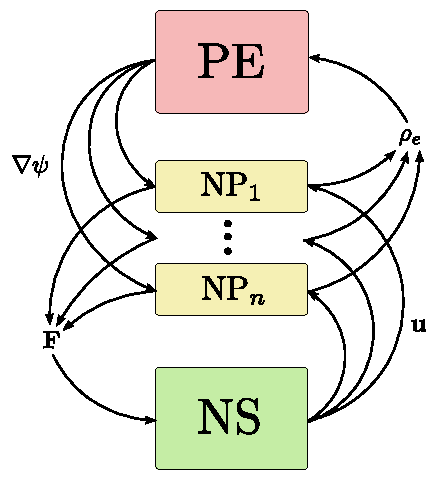
\includegraphics[width=0.5\textwidth]{fig/coupling.pdf}
\end{center}
\caption{Visualisation of the coupling between the three equations
  present in the model. Poisson's equation (PE), The set of
  Nernst-Planck equations (NP$_1$ ... NP$_n$) and the Navier-Stokes
  equations (NS). The dependencies have also be marked with arrows
  indicating what quantities for a certain equation that are needed
  from an other.}
\end{figure}


\section{The potential - Poisson's equation}\label{sec:et:poisson}
To be able to model the flow dynamics of liquids in a channel with
present EDLs, the potential and charge distribution
in the channel must be determined. These quantities are mutually
related through Poisson's equation for electrostatics:

\begin{equation}\label{eq:pb}
\nabla^2\psirm = -\frac{\rho_e}{\epsilon_r \epsilon_0}
\end{equation}
where $\psirm$ is the electrical potential, $\rho_e$ the electrical
charge density, $\epsilon_r$ is the relative permittivity and
$\epsilon_0$ the vacuum permittivity. Under certain assumptions, the
charge density may be explicitly determined as a function of the
potential distribution, one such result is the so called
Poisson-Boltzmann equation, further discussed in section \ref{sec:et:pb}.

\subsection{Boundary conditions}
At the charged boundaries, most physical situations may be covered by
either specifying the potential or the surface charge density. The
former would be a boundary condition of Dirichlet type:

\begin{equation}
\psirm(\x) = \zeta(\x)\;,\;\; \x \in \Gamma
\end{equation}
and the latter a boundary condition of Neumann type:

\begin{equation}\label{eq:et:fix_c}
\nabla\psirm(\x) \cdot \n =
-\frac{\sigma(\x)}{\epsilon_0\epsilon_r}\;,\;\; \x \in \Gamma
\end{equation}
where $\Gamma$ denotes the boundary of the domain and $\n$ is the
normal to the boundary surface.\- \cite{hlushkou}


\section{The transport of charges - Nernst-Planck equation}
The charge concentration in an electrolyte is indeed affected by its
environment. In the model proposed here, influences from: advection of
the electrolyte, diffusion due to concentration gradients and effects
from the electric field originating from charged objects placed at the
border or in the flow is considered. Charge conservation without any
external sources of the ion density, $\mathrm{C}(\x, t)$ gives:

\begin{equation}\label{eq:charge_conc}
\dfrac{\partial \C}{\partial t} + \nabla \cdot \J = 0
\end{equation}
where $\mathbf{J(\mathbf{x}, \mathrm{t})}$ is the net flux induced
by the effects described above. Explicit expressions for the fluxes
due to advection and diffusion respectively are 

\begin{equation}
\J_{adv} =
\C\ubf
\end{equation}
and 
\begin{equation}
\mathbf{J}_{dif} = -D\nabla \mathrm{C} 
\end{equation}
where $\mathbf{u}$ is the advective velocity and $D$ is the diffusion
coefficient. The ionic flux due to the presence of an electric
potential, $\psirm(\x, t)$, is given by the Nernst equation
\cite{dongquing-ren-book}:

\begin{equation}
\J_{ele} = -\frac{zq_eD}{k_BT}\C\nabla\psirm
\end{equation}
where $z$ is the relative charge of an ion, $q_e$ is the fundamental
charge, $k_B$ is the Boltzmann constant and $T$ is temperature of the
fluid.

Summing up the fluxes and putting them into eq. \eqref{eq:charge_conc} gives


\begin{equation}\label{np}
\dfrac{\partial \C}{\partial t} = \nabla \cdot \left [
 D\nabla \mathrm{C} - \C\ubf + \frac{zq_eD}{k_BT}\C\nabla\psirm
\right]
\end{equation}
which is a known result often referred to as the Nernst-Planck
equation. The advective velocity, $\ubf$, and the potential gradient,
$\nabla \psirm$, are obtained from couplings to the Navier-Stokes and
Poisson's equations respectively. More about the coupling between the
equations will be discussed in section \ref{et:coupling}.

\subsection{Boundary conditions}
Depending on the physical situation that is being modelled, different
conditions may be imposed at the boundaries of the domain. Throughout
this work, at hard boundaries (walls), the charge flux out of the
boundary will be set to zero, i.e.:

\begin{equation}
\J \cdot \mathbf{n}\big|_{x \in \Gamma} = 0 
\end{equation}
where $\mathbf{n}$ denotes the normal to the surface and $\Gamma$ is
the boundary of the domain. 


%what we need

%nernst planck


%poisson boltzmann steady state, fix potential 

\subsection{Poisson-Boltzmann equation}\label{sec:et:pb}
Consider a system consisting of an electrolyte in contact with a
(flat) charged wall.  Under certain assumptions, it is possible to
explicitly determine the charge density in eq. \eqref{np} as a
function of the electric potential. E.g. if there is no advection
present and if the system has reached a steady state, i.e. $\partial
\C /\partial t = 0$ and $\ubf = \mathbf{0}$ we have:

\begin{equation}\label{pb_constant_flux}
D\nabla \mathrm{C} + \frac{zq_eD}{k_BT}\C\nabla\psirm = \alpha
\end{equation} 
where $\alpha$ is some arbitrary constant. Due to the steady state
assumption, what the equation above actually says is that the net flux
of charge in the system is constant. Since no flux of charge is wanted
to flow through the wall boundary, the flux is set to zero on the wall
and since the flux is constant it will therefore be zero everywhere in
the liquid, i.e. $\alpha = 0$.

Considering only a one-dimensional situation with a position variable
$y$ varying in a direction out from the wall into the liquid,
eq. \eqref{pb_constant_flux} reads

\begin{equation}\label{eq:pb_eq_for_C}
\frac{1}{\C} \dfrac{d \C}{d y} + \frac{zq_e}{k_BT} \dfrac{d \psirm}{d
  y} = 0.
\end{equation}

The charge density is determined by solving eq. \eqref{eq:pb_eq_for_C}
for $\C$, i.e. integrating the equation. In order to avoid introducing
additional unknown quantities, the equation is integrated to far away
from the wall where the potential from the EDL is assumed to have
decreased to zero and where the concentrations, $\C^{\infty}$, of the
electrolyte is known.

\begin{equation}
\int_y^{\infty} d\ln( \C(y')) = -\frac{z q_e}{k_BT}\int_y^{\infty}d\psirm(y')
\end{equation}
This gives an expression for $C(y)$:

\begin{equation}\label{eq:C}
\C(y) = \C^{\infty} \exp\left(-\frac{z q_e \psirm(y)}{k_BT}\right).
\end{equation}

In a general case, there may be several species of ions in the
electrolyte, the net charge density, $\rho_e$, is then given by simply
summing up the contributions from the different species:

\begin{equation}\label{eq:rho}
\rho_e = q_e\sum_i z_i \C_i.
\end{equation}

Summarising eqs. \eqref{eq:pb}, \eqref{eq:C} and \eqref{eq:rho} gives
the Poisson-Boltzmann equation in one dimension

\begin{equation}\label{eq:pb_real}
\dfrac{d^2\psirm(y)}{dy^2} = -\frac{q_e}{\epsilon_r \epsilon_0}\sum_i z_i
\C_i^{\infty} \exp\left(-\frac{z_i q_e \psirm(y)}{k_BT}\right).
\end{equation}

\subsubsection{The Debye–Hückel approximation}
Historically, the non-linear nature of eq. \eqref{eq:pb_real}
complicated when it came to solving it. This was a major difficulty in
the past when the computational power at hands were rather limited. A
linearisation is therefore sometimes done, this linear version of the
PB equation is often referred to as the Debye–Hückel
approximation. The solution of the linearisation gives however,
something to compare with and will be used when defining a
characteristic length scale of the EDL.

For a 1:1 electrolyte solution, eq. \eqref{eq:pb_real} reduces to

\begin{equation}
\frac{d^2\psi(x)}{dx^2} = \frac{2n^{\infty}q_ez}{\epsilon_r
  \epsilon_0}
\sinh\left(\frac{z q_e \psi(x)}{k_BT}\right).
\end{equation}
and the linearised equation is

\begin{equation}
\frac{d^2\psi(x)}{dx^2} = \frac{2n^{\infty}q_e^2z^2}{\epsilon_r
  \epsilon_0 k_B T} \psi(x) = \kappa^2 \psi(x)
\end{equation}
where $\kappa^{-1}$ is the Debye length and gives a measure for the
characteristic size of the EDL.

\subsubsection{Limitations of the Poisson-Boltzmann model}
As the Poisson-Boltzmann equation is derived several assumptions are
made. First, the net flux of ions are assumed to be zero and that the
advective contribution the flux is negligible. Thus, the PB equation is
only applicable when the system is at (or very close) thermodynamical
equilibrium.

\todo{Continue this discussion...}


%% In this work, flows of ionic solution will be studied and the
%% assumption with thermodynamical equilibrium does not apply. However
%% for low-speed flows the model may still be a decent approximation,
%% which will be investigated.

%% The second assumption, may also stay unfulfilled in some cases
%% investigated here. The fluid in contact with the wall must be of
%% substantial size in relation to the EDL thickness. There will be
%% cases where the choice of $\zeta$ potential in combination with thin
%% channels will make this assumption not fulfilled.

%% Since the PB equation is unable to model the system of
%% interest, a different approach will be presented. However, throughout
%% this work, references and comparisons with the PB model w
%% ill be made. 


%intro

%liten härledning av högerledet 
%diffusion by conc grad. = grad of
%potential <==> termodynamic equilibrium
%chem pot definerad som....
% eq.
% boundary conditions
%antagaganden !!!


%% A simple and commonly used approach for determining potentials (and
%% charge distributions) in systems with present EDLs is by solving
%% eq. \eqref{eq:pb} with a charge distribution of Boltzmann
%% type. Here follows a brief derivation of this term together with some
%% discussion on the assumptions made.

%% The fundamental assumption that the derivation of the charge
%% distribution is based on, is the fact that the system is assumed to be
%% under thermodynamical equilibrium. I.e. forces, acting on the ions,
%% due to chemical diffusion from concentration gradients and from the
%% electrical field are therefore balancing each other. In one dimension:

%% \begin{equation}\label{eq:dif_elec_forces}
%% \frac{d \mu_i}{dx} = -z_i q_e\frac{d\psi}{dx}
%% \end{equation}
%% where $\mu_i$ is the chemical potential for species $i$, $z_i$ is the
%% relative charge of species $i$, $q_e$ the fundamental charge and
%% $\psi$ is the EDL potential. The chemical potential is given by
%% \cite{ren}:

%% \begin{equation}
%% \mu_i = \mu_i^{\infty} + k_BT\ln n_i
%% \end{equation}
%% where $\mu_i^{\infty}$ is a reference value for the chemical potential,
%% here the potential value far from the charged wall is used, $k_BT$ is
%% the thermal energy and $n_i$ is the ion concentration of species
%% $i$. This expression plugged into eq. \eqref{eq:dif_elec_forces} gives

%% \begin{equation}\label{eq:eq_for_ni}
%% \frac{d \ln(n_i)}{dx} = - \frac{z_i q_e}{k_BT}\frac{d \psi}{dx}.
%% \end{equation}


\section{The velocity field - Navier-Stokes equations}\label{sec:et:ns}
In hydrodynamics, the Navier-Stokes equations are one of the most
fundamental corner stones. They describe the motion of a fluid under
the influence of various internal and external forces. 

For later convenience and for reference when it comes to deriving the
Lattice-Boltzmann formulation of the NS equation, a brief sketch of a
derivation will here be presented. A most general form of the
Navier-Stokes equation follows from momentum conservation

\begin{equation}
\dfrac{\partial (\rhorm \ubf)}{\partial t} + \nabla \cdot (\rho \ubf
\otimes \ubf) + \Q = 0 
\end{equation}
where, $\rhorm$ is fluid density, $\ubf$ is velocity and $\Q$ is a
momentum source term (force per volume). Expanding the time
derivative and the divergence terms respectively gives
 
\begin{equation}\label{eq:et:nspre}
\ubf \left ( \dfrac{\partial \rhorm}{\partial t} + \nabla \cdot
  (\rhorm \ubf) \right ) + \rhorm \left (\dfrac{\partial \ubf}{\partial t} +
  \ubf \cdot \nabla \ubf 
  \right ) + \Q = 0.
\end{equation}
By assuring mass conservation (without sources) we have that

\begin{equation}\label{eq:et:mass_conc}
 \dfrac{\partial \rhorm}{\partial t} + \nabla \cdot(
  \rhorm \ubf) = 0
\end{equation}
and eq. \eqref{eq:et:nspre} reduces to

\begin{equation}\label{eq:et:ns_general} 
\rhorm \left (\dfrac{\partial \ubf}{\partial t} +
  \ubf \cdot \nabla \ubf 
  \right ) + \Q = 0
\end{equation}
which together with eq. \eqref{eq:et:mass_conc} is a general
formulation of the Navier stokes equations. 

The force term $\Q$, is determined by the physical properties of the
fluid and from its environment. In this work, only incompressible
Newtonian fluids will be studied. The force contribution to $\Q$
involved in that case is limited to viscous forces, pressure gradients
in the fluid and to external force fields. Putting that into
eqs. \eqref{eq:et:mass_conc} and \eqref{eq:et:ns_general} gives

\begin{equation}\label{eq:et:ns_incompressible}
 \nabla \cdot \ubf = 0
\end{equation}
and

\begin{equation}\label{eq:et:ns_mom}
\rhorm \left (\dfrac{\partial \ubf}{\partial t} +
  \ubf \cdot \nabla \ubf 
  \right ) = - \nabla \Prm  + \mu \nabla^2 \ubf + \F
\end{equation}
where $\Prm$ is the pressure, $\mu$ the kinematic viscosity and $\F$
is the contributions from  external forces.

\subsection{Boundary conditions}

At hard boundaries (walls), the boundary conditions to
eqs. \eqref{eq:et:ns_incompressible} and \eqref{eq:et:ns_mom} are set
on the velocity of either a Dirichlet or Neumann type. In most
physical situations the Dirichlet condition is used which corresponds
to that there is a friction between the fluid and the wall, usually
full friction, i.e. when no relative movement between fluid and wall
is present and the velocity at the wall boundary is set to zero, i.e.

\begin{equation}
\ubf = 0 \;,\;\; \x \in \Gamma
\end{equation} 
where $\Gamma$ denotes the boundary. The Neumann type conditions are
used for no-friction walls where the normal component of the
derivative of the velocity is specified, usually to zero.

At wet boundaries, inlets and outlets, of the domain various boundary
conditions may be set. For instance the pressure or the velocity could
be fixed. In the case of a fixed pressure boundary, a flow direction
must also be specified for completeness. \cite{some fluid dynamics
  text}


\section{Pressure-driven electrokinetic flow}\label{sec:et:streaming_pot}
As a charged fluid is driven by a pressure gradient, a movement of
charges, i.e. an electrical current will be induced. Due to the charge
flux, a potential gradient will build up along the flow
direction. This potential is usually referred to as the streaming
potential, $\phi(\x)$, and its magnitude is determined from the
induced current through Ohm's law

\begin{equation}
\J = -  \sigma \nabla \phi  
\end{equation}   
where $\sigma$ is the conductivity of the fluid. in a perfectly
conducting fluid there will be no potential differences. Also a
complete neutral solution will carry no net current and also in this
case there will be no potential differences.

Charges under the influence of an electric field will be affected by a
force. Charges moving due to this force will, in a liquid, also pull
liquid (uncharged) molecules with them. In a macroscopic limit, the
force density affecting the charges in the liquid is assumed to affect
the liquid as a whole. The volumetric force affecting the fluid from
the presence of the streaming potential is then given by:

\begin{equation}
\F = - \rho_e \nabla \phi
\end{equation}
where $\rho_e$ is the charge density. This is an example of how the
charge density from the Nernst-Planck equation may couple to the force
term in Navier-Stokes equations. 

This force will always be affecting the fluid in a direction opposite
to the net flux of charge, i.e. the force will slow the fluid down,
this is illustrated in fig. \ref{fig:et:ev}. This effect that a moving
net charged fluid is slowed down is called the \emph{electroviscous
  effect}. The name originates from that a similar effect might be
achieved by increasing the viscosity of the fluid.

\begin{figure}
\begin{center}
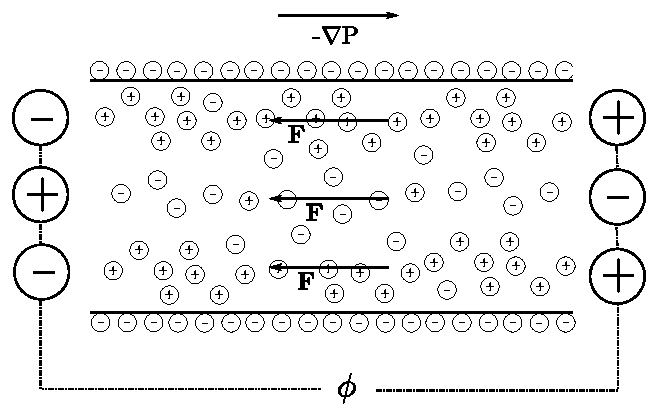
\includegraphics[width=0.7\textwidth]{fig/channel_electroviscous.pdf}
\end{center}
\caption{Example of an electroviscous system. The fluid is driven by a
  pressure gradient, $\nabla \Prm$. The directions of the forces on
  the fluid are always opposite to the flow direction. The force
  originates from the potential difference, $\phi$, that builds up
  along the channel. The force is always opposite to the flow
  direction, thus slowing the flow down.}
\label{fig:et:ev}
\end{figure}


\section{Electroosmotic flow}\label{sec:et:electroosmosis}
Instead of driving the fluid flow through a pressure drop, a net
charged fluid may be driven by an external electric field. This may
be seen as the opposite case to that in section
\ref{sec:et:streaming_pot} where a current is induced by a pressure
drop.

The volumetric force on the fluid from the external field, $\E_{ext}$,
is given by

\begin{equation}
\F = \rhorm_e \E_{ext}
\end{equation}

where $\rho_e$ is the charge density. If the electric field is
constant (or at least has the same direction) everywhere, the sign of
the force is not in the same direction for a net charged positive area
of the fluid as for a net charged negative. Thus the fluid may be
either slowed down or sped up. This is a qualitative difference to
pressure driven situation and is illustrated in fig. \ref{fig:et:eo}.

\begin{figure}
\begin{center}
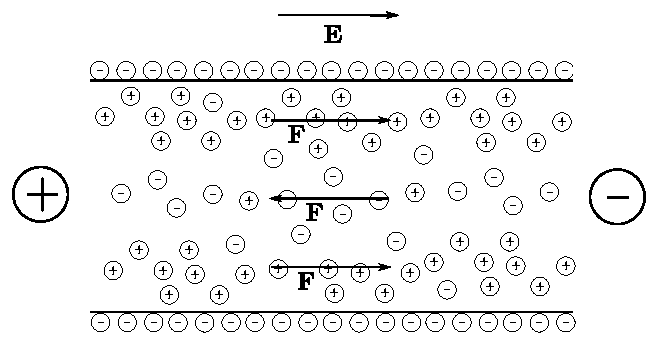
\includegraphics[width=0.7\textwidth]{fig/channel_electroosmosis.pdf}
\end{center}
\caption{Example of an electroosmotic system. The fluid is driven by
  an external electric field, $\E$. The directions of the forces on
  the fluid from the electric field are indicated with arrows. Note
  however that the fluid does not necessarily has to flow in the
  direction of the force, this due to viscous effects in the fluid. }
\label{fig:et:eo}
\end{figure}

The electroviscous effect is in the case of pure electroosmotic flow
usually neglected as the field due to the streaming potential is, in
most physical cases, small in comparison to the applied external
field. \cite{wang-poi}


%lite intro

%börja inte med allmän teoretisk formulering

%sedan lite resultat, double layers

%pressure driven flows...


\chapter{The lattice-Boltzmann method}
Rather than modelling on a macroscopic or microscopic scale, the
lattice-Boltzmann method operates at a scale in between those, often
referred to as a mesoscopic scale. Nowadays, the method is most
frequently used in modelling fluid dynamics, i.e. solving the
macroscopic Navier-Stokes equations. However, the lattice-Boltzmann
method is not limited to this case and may be used to model other
macroscopic systems as well. In this chapter a LBM approach will, in
addition to the Navier-Stokes equations, also be formulated for the
Nernst-Planck and the Poission's equation.

\section{Historical overview}
With the introduction of electronic calculating machines came also a
completely new possibility of tackling problems. New fields of
computational science was born and methods for solving both new and
traditional problems were developed.

The idea of using a discrete and simplified version of the
Boltzmann-equation dates back to the mid 60's \cite{scholarpedia-lbm}
with an experimental attempt to model simple gas dynamics. However, at
the time, this kind of statistical computational approaches was not
considered a serious alternative for the modelling of more
sophisticated and complex systems such as fluid behaviour. It was
first in the mid 80's when Frisch, Hasslacher and Pomeau showed that a
lattice automaton, with a lattice of certain symmetry and that
conserved mass and momentum in the collisions, reproduced the
Navier-Stokes equations in a macroscopic limit. It was by their work
and the always increasing computational power that made the idea of
fluid modelling on a mesoscopic scale a serious research
topic. \cite{wolf-gladrow}

But the lattice gas automata (LGA) approach suffered from some flaws,
e.g. that the boolean nature of the method introduced statistical
noise and that lack of symmetry in the lattices used made the advection
non-isotropic. The statistical noise was usually dealt with by
averaging which resulted in a coarsed domain and the advection issue
was handled by introducing lattices of higher symmetry. As the flaws
of the LGA approach was dealt with one after one, the method evolved
into what we today know as the lattice-Boltzmann method, with the
crucial refinement of using continuous distributions over boolean
variables. \cite{wolf-gladrow} 

Today, the lattice-Boltzmann method is in many situations indeed a
competitor to more traditional CFD methods. For example with
advantages when it comes to parallelisation or implementing boundary
conditions in complex geometries. The downside with the LBM is the
lack of theoretical work done and lack of literature compared to the
case with traditional methods such as finite element/volume
methods. \cite{junk-asym}

\section{Statistical background}\label{sec:lbm:stat}
Consider one litre of air. At NTP, the volume will contain in the
order of $10^{22}$ molecules. In order to model this system
microscopically, 6 variables per molecule will be needed to describe
the microstate of the system. Just to store the state of the system in
a computer would require more space than the estimated size of the
whole world wide web times one million \cite{wolfram-alpha-web}. Thus,
for these kind of systems, the microscopic approach is somewhat
impractical.

For that reason, statistical approaches have been developed for these
kind of problems. A fundamental quantity used for describing the
system is a continuous probability density distribution, $f$. This
distribution may be regarded as an average over the
microstates. Consider a volume of $d^3\x d^3\mathbf{p}$ in phase
space, the number of molecules, $dN$ in this volume is then given
through the density distribution, $f$ as

\begin{equation}
dN(\x, \p, t) = f(\x, \p, t)\drm^3\x \drm^3\p.
\end{equation}
Thus $f(\x, \p, t)$ is a measure for the number of particles at
location $\x$ with momentum $\p$ at time $t$. Macroscopic variables is
obtained by summing, e.g. the particle density, $n$, is obtained from

\begin{equation}
n(\x, t) = \int f(\x, \p, t) \drm^3\p
\end{equation}
and the macroscopic momentum density of the system is determined by

\begin{equation}
\rho(\x, t) \ubf(\x, t) = \int \p f(\x, \p, t) \drm^3\p
\end{equation}
where $\rho = m n$ is the mass density. Multiplying $f$ by a power $k$ of
$\p$ or $\mathbf{v} = \p/m$ and integrating is often referred to as
taking the $k$:th moment of $f$ and is a term that will be used
throughout this chapter.

In the late 19th century, Boltzmann developed a model for the time
evolution of $f$. To do this he had to make several
assumptions. First, only collisions between two particles are
considered, this makes the equation mostly applicable to dilute
gases. Second, the two particles colliding are assumed to be
uncorrelated before the collision. Third, external forces are assumed
not to affect the collisions \cite{wolf-gladrow}. The equation is
named after its father to the Boltzmann (transport) equation and
reads:

\begin{equation}\label{eq:lbm:boltzmann-eq}
\partial_t f + \frac{\p}{m} \cdot \nabla_{\x}f + \frac{\F}{m} \cdot
\nabla_{\mathbf{v}}f = Q(f, f)
\end{equation}
where $f$ is the distribution function for a single species collection
of particles of mass $m$, $\F$ is external forces, $\p$ is momentum,
$\nabla_{\x}$ and $\nabla_{\mathbf{v}}$ are the gradients in location
and velocity space respectively. The right-hand side contains the so
called collision term which in the general case is expressed as an
integral. This integral states how the distribution function changes
after a two particle collision. However, the structure of this
integral is in most physical situations too complicated to be used
directly. Therefore, a number of simplifications have been proposed
during the years.

When designing these approximations, at least two main properties of
the collision integral must be kept. \cite{wolf-gladrow}

\begin{enumerate}
  \item The same quantities that is conserved under collisions in the
    collsion integral must also be conserved in the approximation.
  \item Boltzmann's H-theorem must be fulfilled for the
    approximated collision operator.
\end{enumerate}

Without being to specific, the H-theorem states that the entropy
computed from $f$ is always increasing with time and that the maximum
entropy is obtained for a so called Maxwellian distribution in
momentum/velocity space. Boltzmann used an other quantity denoted by H
closely related to entropy, thus the name of the theorem. The
Maxwellian distribution in two dimensions that $f$ tends towards is
given by

\begin{equation}\label{eq:lbm:maxwell}
f^{(M)}(\x, \mathbf{v}, t) = n \left ( \frac{m}{2 \pi k_B T} \right )
\exp{\left( -\frac{m}{2 k_B T} (\mathbf{v} - \ubf)^2\right)}
\end{equation} 
where $\ubf(\x, t)$ is the mean velocity of the particles in the system and
$n(\x, t)$ is the number of particles at location $\x$. In section
\ref{sec:lbm:col}, one of the most widely used approximations of the
collision integral will be presented.


\section{Basic idea of the LBM}
As previously noted, the lattice-Boltzmann method is a mesoscopic
method. This means that the modelling is neither done on a microscopic
(molecular) level nor by direct solving the macroscopic equations
involved. The aim, in the most situations with the lattice-Boltzmann
method is indeed to solve some macroscopic equation but not
direct. Instead a statistical model is used with various mesoscopic
variables that, in some limit, reproduces the macroscopic
variables. It is also possible to ensure that these variables (to some
extent) fulfil a certain macroscopic equation by using a certain
scheme.

Basically the lattice-Boltzmann method solves a discretised version of
eq. \eqref{eq:lbm:boltzmann-eq} for the distribution functions from
which the macroscopic quantities may be determined. Both the spatial
positions and the velocity space is discretised allowing the
distributions to ``sit'' only at certain positions and to stream to
neighbouring locations only in certain directions. A naive way to
visualise the evolution of $f$ is to consider the distribution
functions at the lattice nodes as pseudo particles that move along the
lattice and collide.

Usually in two dimensions the velocity space is discretised into 9
distinct velocities, more about the choice of lattice is discussed in
section \ref{sec:lbm:lattice}. In this case 9 distribution functions
are needed per node which might correspond to one or two macroscopic
variables but is indeed fewer than the number of variables needed for
a microscopic approach.

The discretised Boltzmann equation is referred to as the
lattice-Boltzmann equation (LBE) and is one of the fundamental corner
stones in the lattice-Boltzmann method, it reads:

\begin{equation}\label{eq:lbm:lbe}
f_i(\x + \cbf_i\delta_t, t + \delta_t) - f_i(\x, t) = \Omega_{ij}(\x, t)
\end{equation}
where $f_i$ denotes the distribution function for direction $\cbf_i$,
$\delta_t$ is the time step and $\Omega_ij$ is the (for now
non-specified) collision operator. An implicit sum over the second
velocity index $j$ is assumed. Various forms of collision operators
exist and will be further discussed in section \ref{sec:lbm:col}.

\subsection{Computational algorithm}
In order to solve eq. \eqref{eq:lbm:lbe} the distribution functions
must be set to some initial value. The choice of initial value is in
most cases crucial with respect to stability and accuracy of the
method. More about the initialisation will be discussed in later
sections of this chapter. 

When a proper initialisation has been performed, the time evolution of
the distribution functions is determined iteratively by the explicit
scheme in the LBE, eq. \eqref{eq:lbm:lbe}. The update in each time
step is usually divided into two computational tasks. First, the new
value that later will be propagated to a neighbouring node is computed,
i.e.

\begin{equation}
f_i^{*}(\x, t + \delta_t) = f_i(\x, t) + \Omega_{ij}(\x, t)
\end{equation}
This step will be referred to as the collision step since it is here
the ``collision'' is computed. The second step consists of propagating
the distribution functions to the neighbouring node in its
corresponding direction, i.e.
\begin{equation}
f_i(\x + \cbf_i\delta_t, t + \delta_t) = f_i^*(\x, t + \delta_t)
\end{equation}
This step will be referred to as the streaming step.

In the case of a finite domain, certain rules (boundary conditions)
must be specified at the boundaries. Typically the distribution
functions that are going to be streamed out of the domain is used to
define the unknown ones that will ``enter'' the domain. More about
boundary conditions in section \ref{sec:lbm:bound}. Thus, at each time
step, the boundary conditions must also be handled. 

This is broadly the whole computational algorithm behind the LBM, in
fig. \ref{fig:lbm:algo}, a flow scheme of the algorithm is shown.

\begin{figure}
\begin{center}
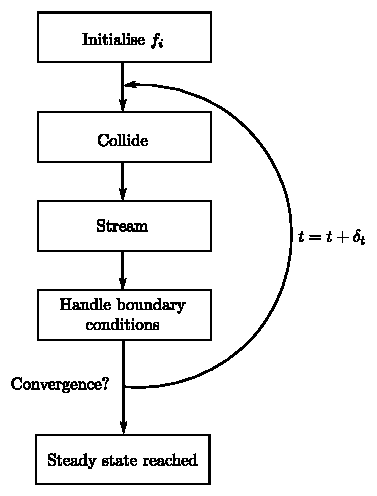
\includegraphics[width=0.5\textwidth]{fig/algorithm.pdf}
\end{center}
\caption{Flowchart of the most fundamental parts in an implementation
  of the LBM. The convergence is usually tested for a macroscopic
  variable.}
\label{fig:lbm:algo}
\end{figure}

\nomenclature{LBE}{Lattice-Boltzmann Equation}


\section{The BGK collision operator}\label{sec:lbm:col}
The collision term in the LBE is the main ingredient in what
determines the physics of the system that is being modelled. Here the
desired interaction of the pseudo particles is stated. In section
\ref{sec:lbm:stat}, two necessary properties to approximations of the
full collision integral was stated.

One of the simplest collision operators that fulfil conditions (1)
and (2) in section \ref{sec:lbm:stat} is the BGK operator (BGK from
its creators: Bhatnagar, Gross and Krook). It was proposed in 1954 and
is today one of the most commonly used collision operators both in the
case of the lattice-Boltzmann and the continuous Boltzmann
equation. It is based on the principle of relaxing $f$ towards a
Maxwellian distribution. The relaxation is also performed in such a
way that the collision invariants are preserved.  In the discrete case,
eq. \eqref{eq:lbm:lbe} the operator is given by:

\begin{equation}\label{eq:lbm:bgk}
\Omega_{ij} = \Omega_i = -\omega \left[ f_i(\x, t) - f_i^{(eq)}(\x, t)
  \right]
\end{equation}
where $\omega$ is a parameter determining the relaxation rate and
$\feq$ should be an equilibrium distribution that makes sure that the
necessary conditions are fulfilled. In the discrete case, a truncated
expansion of eq. \eqref{eq:lbm:maxwell} is typically used
\cite{wolf-gladrow}. This gives for instance


\begin{equation}
\feq = w_i\rho \left [ 1 + \frac{\ci \cdot \ubf}{c_s^2} +
  \frac{(\ci \cdot \ubf)^2}{2c_s^4} - \frac{\ubf^2}{2c_s^2} \right]
\end{equation}
where $w_i$ is a lattice specific weight, $\rho$ is the zeroth moment
of $\fii$ and $\ci$ is a unit velocity in the discretised velocity
space.

The BGK operator is due to its simplicity both when it comes to
theoretical treatment and implementation a popular choice. However in
some physical situations, e.g. multi-phase or high Reynolds-number
flows, more sophisticated alternatives are required
\cite{wolf-gladrow}. Throughout this work, the BGK operator will be
used.

\nomenclature{BGK}{Relaxation type collision operator (Bhatnagar,
  Gross and Krook)}


\section{The lattice}\label{sec:lbm:lattice}
The discrete spatial coordinates together with the discrete velocity
coordinates forms a lattice. Spatial coordinates are neighbourwise
connect through the discrete velocities. The discretisation in the LBM
must be performed in such a way that the lattice may be produced from
translating a single unit cell. This gives that the spatial resolution
is constant for the whole domain. In other approaches, e.g. finite
element methods the mesh may locally be refined at interesting regions
of the domain which is a strength to these methods over the LBM.  

There exist a convention for naming different lattices. A lattice of
dimension $d$ and with $q$ distinct velocities is denoted by
D$d$Q$q$. For example a lattice with 9 velocities in dimension 2 is
denoted D2Q9. An example of two different lattices is presented in
fig. \ref{fig:lbm:lattices}. The D2Q9 lattice is also the one that
will be used in this work, the velocities $\ci$ are given by

\begin{equation}\label{eq:lbm:d2q9_c}
\{\ci\} = \left\{
\begin{bmatrix}0\\0\end{bmatrix}, 
\begin{bmatrix}1\\0\end{bmatrix}, 
\begin{bmatrix}0\\1\end{bmatrix}, 
\begin{bmatrix}-1\\0\end{bmatrix}, 
\begin{bmatrix}0\\-1\end{bmatrix}, 
\begin{bmatrix}1\\1\end{bmatrix}, 
\begin{bmatrix}-1\\1\end{bmatrix}, 
\begin{bmatrix}-1\\-1\end{bmatrix}, 
\begin{bmatrix}1\\-1\end{bmatrix}
\right\} 
\end{equation}

\begin{figure}
  \centering
  \subfloat[D2Q7
    ]{\label{fig:lbm:q7}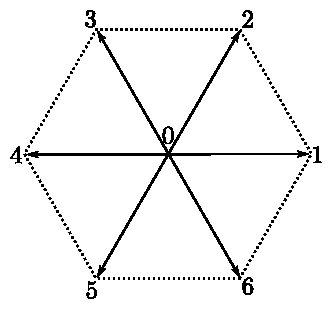
\includegraphics[width=0.4\textwidth]{fig/lattice_d2q7-crop.pdf}}      
  \hspace{15pt} \subfloat[D2Q9
  ]{\label{fig:lbm:q9}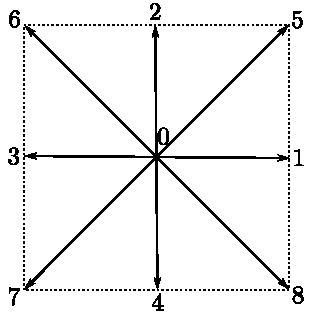
\includegraphics[width=0.35\textwidth]{fig/lattice_d2q9.pdf}
  }
  \caption[Two different unit cells for lattices used in the LBM in two
    dimensions.]{Two different unit cells for lattices used in the LBM in two
    dimensions. In (a) the D2Q7 seven speed lattice is shown and in
    (b) the nine speed D2Q9 lattice. The numbering at the edges is the
    usual naming convention for the different velocities.}
  \label{fig:lbm:lattices}
\end{figure}
 
To be able to retrieve the desired equations in the macroscopic limit
of the LBE, the lattice used must possess a certain degree of
isotropy. Thus the choice of lattice is not arbitrary. For instance,
for obtaining the Navier-Stokes equations, the lattice velocities must
at least posses the following properties:

\begin{subequations}\label{eq:lbm:i0}\label{eq:lbm:i1}\label{eq:lbm:i2}\label{eq:lbm:i3}\label{eq:lbm:i4}
\begin{align}
\sum_i w_i &= 1\\
\sum_i w_ic_{i\alpha} &= 0 \\
\sum_i w_ic_{i\alpha}c_{i\beta} &= c_s^2\delta_{\alpha \beta}\\
\sum_i w_ic_{i\alpha}c_{i\beta}c_{i\gamma} &= 0\\
\sum_i w_ic_{i\alpha}c_{i\beta}c_{i\gamma}c_{i\delta} &= c_s^4(\deltasec)
\end{align}
\end{subequations}

%\begin{equation}\label{eq:lbm:i5}
%\sum_i w_ic_{i\alpha}c_{i\beta}c_{i\gamma}c_{i\delta}c_{i\kappa} = 0
%\end{equation}

where the sums are over the discrete velocities $\ci$, $w_i$ are
lattice specific weights $c_s$ is the speed of sound for the lattice
and $\delta_{ij}$ is a Kroenecker delta. 

The weights are introduced to compensate for the fact that different
velocity vectors are of different length. See for example the
D2Q9 lattice in fig. \ref{fig:lbm:q9} where three lengths are
present. In this case, three different weights will be needed. From
the relations in eqs. \eqref{eq:lbm:i1} follow that
these weights are: 
\begin{equation}\label{eq:lbm:weights}
w_i = 
\left\{
  \begin{array}{l l}
    4/9 & \quad \text{if $i = 0$}\\ 
    1/9 & \quad \text{if $i = 1, 2, 3, 4$}\\    
    1/36 & \quad \text{if $i = 5, 6, 7, 8$}\\
  \end{array} \right.
\end{equation}
The quantity $c_s$ which often is referred to as the speed of sound
may be thought of as an effective propagation velocity of the lattice
and is determined, for the D2Q9 lattice, to

\begin{equation}
c_s = c/\sqrt{3}
\end{equation} 
where $c = |\mathbf{c}_{1,2,3,4}| = \delta_x/\delta_t$.

\nomenclature{D2Q9}{2D lattice with 9 discrete velocities}


\section{Asymptotic analysis}\label{sec:lbm:asym}
Methods from asymptotic analysis will, in this section, be used to
investigate the macroscopic limit of the general LBE. Detailed and
specific analyses for the three different equations considered will be
presented in sections \ref{sec:lbm:asym_np}, \ref{sec:lbm:asym_ns} and
\ref{sec:lbm:asym_pe}. Asymptotic analysis is basically about
describing mathematical objects in some limit, e.g. how a function
behaves for large or small values of some parameter. Consider for
example the series expansion of $\exp(\epsilon)$:

\begin{equation}
\exp(\epsilon) = 1 + \epsilon + \epsilon^2/2 + \epsilon^3/6 + \mathcal{O}(\epsilon^4) 
\end{equation}
It is clear that for sufficiently small values of $\epsilon$, the
terms of higher order is negligible to those of lower order and the
series may be truncated at some point and still be a good
approximation of the expression.

There are different approaches to go from the discrete LBE to a
continuous macroscopic equation. The most frequently applied one to
obtain the Navier-Stokes equations is the Chapman-Enskog method
\cite{junk-boundary}, which will reproduce the compressible
equations. An other method, often employed by M. Junk and his
associates e.g. in \cite{junk-asym}, is a method based on regular
asymptotic expansions, this is the method that will be utilised in
this work and will in the case of Navier-Stokes reproduce the
incompressible equations. A brief discussion of the differences between
the Chapman-Enskog and the regular expansion approaches will be carried
out at the end of this section.

The basic idea behind the analysis is to expand the distribution
function $\fii$ in some small parameter, $\epsilon$. Also this
parameter will be related to the spatial and time scales. The
macroscopic limit is obtained by taking the taylor expansion of the
discrete LBE and comparing terms of equal order in
$\epsilon$. Together with the fact that certain quantities is
invariant under collisions, macroscopic differential equations is
obtained. Now follows the part of the analysis which is common for the
three equations, the more equation specific analysis is carried out in
sections \ref{sec:lbm:asym_np}, \ref{sec:lbm:asym_ns} and
\ref{sec:lbm:asym_pe} respectively.

\subsection{Motivation of the choice of expansion parameter}
The expansion parameter should be a small dimensionless number. If the
lattice is dense enough with respect to the characteristic length
scale of the system, a suitable choice is the Knudsen number which is
defined as the ratio of the mean free path, $\delta_x$, and the
characteristic length of the system under consideration, $\ell_0$,
i.e. $\epsilon = \delta_x /\ell_o$. To be able to perform the
asymptotic analysis we must also relate the time scale to this
parameter. From the fact that the lattice speed $c_s =
\delta_x/\delta_t$ and by introducing a characteristic speed, $u_o =
\ell_0/t_0$, we have

\begin{equation}\label{eq:lbm:rel}
\epsilon = \frac{\delta_x}{\ell_0} = \frac{c_s}{u_0}\frac{\delta_t}{t_0}
\end{equation}
It is now clear that what determines the relation between the
timescale and the parameter $\epsilon$ is the ratio of the
characteristic speed and the lattice speed which is usually referred
to as the Mach number, Ma. In our particular case we will operate in
the incompressible limit, i.e. Ma $\ll$ 1 and a suitable choice is a
small number, thus Ma = $\epsilon$ is chosen \cite{junk-boundary}. The
discretisation of the space and time step is then

\begin{equation}
\delta_x'^2 = \delta_t' = \epsilon^2
\end{equation}
where the primes denote dimensionless variables. This particular
scaling is usually referred to as diffusive scaling.

\subsection{Expanding the LBE}
The LBE, eq. \eqref{eq:lbm:lbe}, with dimensionless variables and the
BGK collision operator reads:

\begin{equation}\label{eq:lbm:nodim_lbe}
f_i(\x' + \epsilon \cbf_i', t' + \epsilon^2) - f_i(\x', t') = -\omega \left[
  f_i(\x', t') - f_i^{(eq)}(\x', t') \right].
\end{equation} 
The primes denoting dimensionless variables will, for readability
reasons, from hereon be dropped. If nothing else is stated we always
consider dimensionless variables.

To obtain a differential equation, the difference equation in
eq. \eqref{eq:lbm:nodim_lbe} is taylor expanded, which gives

\begin{equation}\label{eq:lbm:taylor_lbe}
\ep(\pd\fii) + \ep^2 (\partial_t\fii + (\pd \fii)^2/2 ) + \ep^3
(\partial_t (\pd\fii) + (\pd\fii)^3/6) + \bigO{\ep^4} = 
-\omega \left[
  f_i - f_i^{(eq)} \right]
\end{equation}
Expanding also $\fii$ and $\feq$ in the parameter $\epsilon$:

\begin{equation}\label{eq:lbm:fi_exp}
\fii = \fie{0} + \ep\fie{1} + \ep^2\fie{2} + \ep^3\fie{3} + \bigO{\ep^4}
\end{equation}

\begin{equation}\label{eq:lbm:fi_eq_exp}
\feq = \feqe{0} + \ep\feqe{1} + \ep^2\feqe{2} + \ep^3\feqe{3} +
\bigO{\ep^4}
\end{equation}
and inserting these expressions into eq. \eqref{eq:lbm:taylor_lbe}
gives an equation with terms of varying orders of $\ep$. Separating
this equation in equations of common orders allows for an analysis of
what happens at different scales of $\epsilon$. For the four leading
orders in $\ep$ we have:

\begin{equation}\label{eq:lbm:ep0}
\ep^0:\;\; 0 = -\omega \left[
  \fie{0} - \feqe{0} \right],
\end{equation}

\begin{equation}\label{eq:lbm:ep1}
\ep^1:\;\; \pd\fie{0} = -\omega \left[
  \fie{1} - \feqe{1} \right],
\end{equation}

\begin{equation}\label{eq:lbm:ep2}
\ep^2:\;\; \pd\fie{1} + \partial_t\fie{0} + (\pd \fie{0})^2/2 =
-\omega \left[ \fie{2} - \feqe{2} \right]
\end{equation}
and
\begin{equation}\label{eq:lbm:ep3}
\ep^3:\;\; \pd\fie{2} + \partial_t\fie{1} + (\pd \fie{1})^2/2 +
\partial_t (\pd\fie{0}) + (\pd\fie{0})^3/6 = -\omega \left[ \fie{3} -
  \feqe{3} \right].
\end{equation}

The idea is now that for an equation of a particular order in $\ep$,
use collision invariants and eliminate unknown $\fie{n}$:s by using
equations of lower order in $\ep$. This will in the end result in
differential equations of macroscopic variables, given by moments of
the $\fii$:s.


\section{LBM for the Nernst-Planck equation}\label{sec:lbm:np}
The method presented here is based on representing the Nernst-Planck
equation, eq. \eqref{eq:et:np}, as an equation of advection-diffusion
type. Considering the quantity:  

\begin{equation}\label{eq:lbm:eff_adv}
\bar{\ubf} = \ubf -
  \frac{zq_eD}{k_BT}\nabla\psirm
\end{equation}
as an effective advective velocity, we have:

\begin{equation}\label{eq:lbm:adv-dif}
\dfrac{\partial \rho}{\partial t} + \nabla \cdot ( \bar{\ubf} \rho -
  D\nabla \rho ) = 0
\end{equation}
which is a mass conservation equation with fluxes from diffusion and
from advection respectively. The letter $\C$ for denoting the charge
concentration has in this section been replaced by the letter $\rho$
to avoid the risk of confusing it with the lattice velocities
which traditionally are denoted by ${\ci}$.

A collision operator of BGK type, eq. \eqref{eq:lbm:bgk} will be used
together with a D2Q9 lattice. The lattice-Boltzmann equation then
reads:

\begin{equation}
f_i(\x + \cbf_i\delta_t, t + \delta_t) - f_i(\x, t) = -\omega \left[ f_i(\x, t) - f_i^{(eq)}(\x, t) \right]
\end{equation}
with $\{\cbf_i\}_{i=0}^{Q-1}$ for the D2Q9 lattice as in
eq. \eqref{eq:lbm:d2q9_c}. The equilibrium function, $\feq$, is chosen
as \cite{alexey-tobias}:

\begin{equation}\label{eq:lbm:np_feq}
\feq = w_i \rho \left ( 1 + \frac{\ci \cdot \ubar}{c_s^2} \right)
\end{equation}
with the weights, $w_i$, as in eq. \eqref{eq:lbm:weights}. The charge
density and charge flux density is obtained by taking the zeroth and
first moments of the distribution function respectively, i.e:

\begin{equation}\label{eq:lbm:rho_mom}
\rhorm = \sum_i \fii
\end{equation}
and
\begin{equation}\label{eq:lbm:j_mom}
\jj = \sum_i \fii \ci
\end{equation}
The diffusion constant, $D$, is related to the relaxation parameter
$\omega$ through 

\begin{equation}\label{eq:lbm:np_D}
D = c_s^2 \left( \frac{1}{\omega} - \frac{1}{2} \right).
\end{equation}

\subsection{Asymptotic analysis}\label{sec:lbm:asym_np}
To motivate the appearance of the above suggested method for solving
eq. \eqref{eq:lbm:adv-dif} and for showing under what premises the
method is valid, the macroscopic limit of the discrete scheme will now
be analysed in an asymptotic manner. Note that for the advection
diffusion equation mass is but flux is not conserved.

From the expansion of $\fii$ in eq. \eqref{eq:lbm:fi_exp} and from
eqs. \eqref{eq:lbm:rho_mom} and \eqref{eq:lbm:j_mom} follow the
expansions of the mass density and flux respectively as

\begin{equation}\label{eq:lbm:rho_exp}
\rho = \rhoe{0} + \ep\rhoe{1} + \ep^2\rhoe{2} + \ep^3\rhoe{3} + \bigO{\ep^4}
\end{equation} 
and

\begin{equation}
\jj = \je{0} + \ep\je{1} + \ep^2\je{2} + \ep^3\je{3} + \bigO{\ep^4}
\end{equation} 
The advective velocity is also expanded as: 

\begin{equation}
\ubar = \ubare{0} + \ep\ubare{1} + \ep^2\ubare{2} + \ep^3\ubare{3} + \bigO{\ep^4}
\end{equation}
By plugging these expansion into the equilibrium distribution
eq. \eqref{eq:lbm:np_feq}, the expansion in
eq. \eqref{eq:lbm:fi_eq_exp} is obtained. The terms of order zero is
used in the zeroth order equation of the LBE, eq. \eqref{eq:lbm:ep0},
which gives

\begin{equation}
\fie{0} = w_i\rhoe{0} \left( 1 + \frac{\ci \cdot \ubare{0}}{c_s^2} \right).
\end{equation}
However, since we are only considering advection in the low Mach
limit, i.e. $|\ubar| \sim \ep$, we will in this analysis assume that
$\ubare{0} = 0$. $\ubar$ will then be of order $\ep$ to leading
order. It is possible to show \cite{junk-asym} that this assumption
holds if $\ubar$ is initialised properly, i.e. small and if no major
momentum sources are present. Thus the expression for $\fie{0}$
reduces to

\begin{equation}\label{eq:lbm:np_fi0}
\fie{0} = w_i\rhoe{0}.
\end{equation}

We now continue to the equation of order one in $\ep$,
eq. \eqref{eq:lbm:ep1}. Taking the zeroth moment gives the equation $0
= 0$ which indeed is true but not very useful. Note that the right
hand side vanishes due to mass conservation. $\fie{1}$ will be needed
in the next step and is, by using eq. \eqref{eq:lbm:np_fi0}:

\begin{equation}
\fie{1} = -\frac{1}{\omega} (\pd)(w_i\rhoe{0}) + w_i\left( \rhoe{1} +
\rhoe{0} \frac{\ci \cdot \ubare{1} }{c_s^2} \right).
\end{equation}
Taking the first moment of $\fie{1}$ gives the leading order in the
flux ($\je{0} = 0$ since $\ubare{0} = 0$):

\begin{equation}
\je{1} = \rhoe{0}\ubare{1} - c_s^2/\omega\nabla\rhoe{0}
\end{equation} 

Continuing to the equation of order two in $\ep$,
eq. \eqref{eq:lbm:ep2} and taking the zeroth moment of the equation
gives

\begin{equation}
\nabla \cdot \je{1} + \partial_t \rhoe{0} + c_s^2/2\nabla^2 \rhoe{0} = 0
\end{equation}
and by inserting the expression for $\je{1}$ we end up with

\begin{equation}
\partial_t \rhoe{0} + \nabla \cdot \left [ \rhoe{0}\ubare{1} - c_s^2
  \left( \frac{1}{\omega} - \frac{1}{2} \right)\nabla\rhoe{0} \right ]
= 0
\end{equation}
which is an advection diffusion equation with a diffusion constant as
in eq. \eqref{eq:lbm:np_D}. Since $\rhoe{0}$ fulfils the equation of
interest, the solution $\rho$ that we get from the lattice-Boltzmann
method is at least of first order accuracy. To determine the exact
order of accuracy, higher order terms, $\rhoe{k > 0}$, must be
determined. If also all those terms would be zero the method would be
exact, unfortunately that is not the case. The analysis of higher order
terms will not be performed here, but it is possible to show that
$\rhoe{1}$ is zero only under certain premises, i.e. for a proper
initialisation \cite{alexey-tobias}. $\rhoe{2}$ is however in general
non-zero and the obtained solution is thus second order accurate.  


\section{LBM for Navier-Stokes}
\subsection{Asymptotic analysis}\label{sec:lbm:asym_ns}

\subsection{Forcing schemes}
how to add a ''forcing'' term in the method.

\section{LBM for Poisson's equation}
As Poisson's equation, eq. \eqref{eq:pb}, is considered, a fundamental
difference to the Nernst-Planck and Navier-Stokes equations is
imediatley noted. It is not a differential equation of parabolic but
of elliptic type. If we consider what has been said about the LBM so
far in this chapter, it seems that it is a method that deals with
parabolic equations and not elliptic. However, by introducing a time
derivative to the Poisson's equation and only considering the steady state
solution the LBM may be used even for this equation. A diffusion-like
equation with a source term is then obtained

\begin{equation}\label{eq:lbm:poi_dif}
\partial_t\rho + \nabla^2 \rho = \R
\end{equation}
where $\R$ is the right-hand side of the Poisson's equation.

A LBM for this equation will now be formulated. The LBE to be solved
in this case is, an equation of the form:

\begin{equation}
f_i(\x + \cbf_i\delta_t, t + \delta_t) - f_i(\x, t) = -\omega \left[
  f_i(\x, t) - f_i^{(eq)}(\x, t) \right] + \Gi(\R)
\end{equation}
where $\Gi(\R)$ is an addition to the BGK collision operator to account
for the source term $\R$ in eq. \eqref{eq:lbm:poi_dif}. The equilibrium
distribution is given by

\begin{equation}
\feq = w_i \rho
\end{equation}
where $w_i$ are the weights in eq. \eqref{eq:lbm:weights}.

The quantity $\rho$ which in this work is interpreted to electric
potential in the steady state is determined by

\begin{equation}
\rho = \sum_i \fii
\end{equation}
and the quantity which, to us, is of even more interest, i.e. the
electric field, is given by

\begin{equation}
\nabla \rho = - \frac{\omega}{c_s^2 \delta_x} \sum_i \fii \ci.
\end{equation}
Finally, the addtional source term in the collision operator, $\Gi(\R)$,
is given by

\begin{equation}\label{eq:lbm:gi}
\Gi(\R) = w_ic_s^2 \left( \frac{1}{2} - \frac{1}{\omega} \right)\R.
\end{equation}

\subsection{Asymptotic analysis}\label{sec:lbm:asym_pe}
The given method for solving eq. \eqref{eq:lbm:poi_dif} will now be
motivated by preforming an asymptotic analysis of the suggested LBE.

$\fii$ is expanded as in eq. \eqref{eq:lbm:fi_exp} which gives an
expansion of $\rho$ as in eq. \eqref{eq:lbm:rho_exp}. Further, 
the source term $\R$ is expanded: 

\begin{equation}\label{eq:lbm:R_exp}
\R = \Rexp{0} + \ep\Rexp{1} + \ep^2\Rexp{2} + \ep^3\Rexp{3} + \bigO{\ep^4}
\end{equation} 
which also gives an expansion for the LBE source term as

\begin{equation}\label{eq:lbm:G_exp}
\Gi = \Gie{0} + \ep\Gie{1} + \ep^2\Gie{2} + \ep^3\Gie{3} + \bigO{\ep^4}.
\end{equation} 

The equilibrium distribution is expanded by plugging in the expansion
of $\rho$ from eq. \eqref{eq:lbm:rho_exp}. This gives for the zeroth
order equation in $\ep$, eq. \eqref{eq:lbm:ep0} that

\begin{equation}
\fie{0} = w_i\rhoe{0} + \frac{1}{\omega}\Gie{0}
\end{equation}
However, taking the first moment of the equation gives $\Gie{0} = 0$
and the above expression for $\fie{0}$ reduces to

\begin{equation}
\fie{0} = w_i\rhoe{0}.
\end{equation}

Coninuing to the equation of first order in $\ep$,
eq. \eqref{eq:lbm:ep1} and taking the zeroth moment gives that also
$\Gie{1} = 0$. Taking the first moment of the same equation  gives

\begin{equation}
\nabla \rhoe{0} = - \frac{\omega}{c_s^2} \sum_i \fie{1} \ci \approx -
\frac{\omega}{c_s^2 \delta_x} \sum_i \fii \ci
\end{equation}
Here, for the approximation, the expansion of $\fii$ is used together
with the fact that $\ep = \delta_x$ in dimensionless variables.

The next equation in $\ep$, i.e. the one of order two, will
eventually give us what we are looking for. Taking the zeroth moment
gives

\begin{equation}
-\frac{c_s^2}{\omega} \nabla^2 \rhoe{0} + \partial_t \rhoe{0} +
\frac{c_s^2}{2}\nabla^2 \rhoe{0} = \sum_i \Gie{2}(\Rexp{2})
\end{equation}
From this equation, it is deduced that in order to obtain Poisson's
equation in a steady state situation, i.e. when $\partial_t \rhoe{0} =
0$ the right-hand side must fulfill the follwong condition

\begin{equation}
\sum_i \Gie{2}(\Rexp{2}) = c_s^2\left( \frac{1}{2} - \frac{1}{\omega} \right)\Rexp{2}
\end{equation}
One such $\Gie{2}(R)$ is the one described in eq. \eqref{eq:lbm:gi}. 


\section{Algorithm/Scheme for solving the coupled equations}
the iterative scheme used.

\section{Boundary conditions}\label{sec:lbm:bound}
discussion and description of the boundary conditions
\subsection{bounce back}
accuracy, e.g. second order accurate if placed between node planes...
\subsection{slip}
\subsection{he-zou, constant density/velocity}
\subsection{Maybe something on non-local boundary conditions}

\section{Physical units vs lattice units}
how to interchange between them... etc...

\section{Chapman-Enskog vs regular expansion analysis}


\chapter{A few notes on high performance computing}
intro what is said below refer to computers of a certain
architecture... 

\section{The pipeline}
keep it full.

\section{Locality}
using the caches in a good way. some examples of its importance. 
\subsection{Locality and LBM}

\section{Parallelisation}
shared memory, distributed memory...

data dependence, LBM good!

OpenMP/MPI

\section{Maybe something about profiling}
men kanske inte tillför något vettigt.

\section{Choice of programming language}

\section{Some stats on the performance of the code...}
Lattice updates/s


\chapter{Model benchmarks}
intro 2D

\section{Poiseuille flow}
First out for evaluating the LBM solver of the Navier-Stokes equations
is the situation with Poiseuille flow. This is a classic example and
one of the easiest situations were the NS equations are exact
solvable. Consider a 2D channel of length $l$ and width $H$. If the
flow in this channel is driven by a constant force, e.g. a constant
pressure drop, the velocity profile will adopt to a parabolic shape in
the steady state situation. Here follows a brief derivation of the
exact expression for the velocity profile.

Consider the (non-dimensional) Navier-Stokes
eqs. \eqref{eq:lbm:non-dim-ns} and \eqref{eq:lbm:non-dim-massconc} in
2D. Let $x$ be the direction along the channel and $y$ the direction
across the channel. In the case of a pressure gradient in the $x$
direction and no other external forces involved we deduce that the $y$
component of the velocity is zero. Thus eq. \eqref{eq:lbm:non-dim-ns}
reduces to an equation for the $x$ component of the velocity

\begin{equation}
\dfrac{\partial \ux}{\partial t} - \ux \dfrac{\partial \ux}{\partial
  x} = \frac{1}{\Rerm} \dfrac{\partial^2 \ux}{\partial y^2} -
\dfrac{\partial \Prm}{\partial x}.
\end{equation}
 
Under the assumption of a system in a steady state, i.e. ${\partial
  \ux}/{\partial t} = 0$. Further if the flow is fully developed
${\partial \ux}/{\partial x} = 0$, this also assures that
\eqref{eq:lbm:non-dim-massconc} is fulfilled. We now have together
with writing the constant pressure gradient as $\Delta \Prm/l$

\begin{equation}
\dfrac{\partial^2 \ux}{\partial y^2} =
\dfrac{\Rerm\; \Delta\Prm}{l}.
\end{equation}

Solving this eq. with no slip boundary conditions, $\ux(0) = \ux(H) =
0$ gives an expression of the velocity profile

\begin{equation}\label{fig:mb:ana_poi}
\ux(y) = \dfrac{\Rerm\; \Delta\Prm}{2l}y(y - H).
\end{equation}

The benchmark of the LBM solver of the NS equation described in
section \ref{sec:lbm:ns} was performed with a pressure gradient
incorporated as a force. Other possibilities would be to drive the
fluid by imposing fixed pressures/velocities at the inlet and outlet.
In this case, with a driving force, periodic boundary conditions were
imposed at the inlet and outlet. At the channel walls, the bounce-back
boundary condition described in section \ref{lbm:bb} was imposed. The
actual boundary will thus be located half a node-node distance into
the fluid.

A grid with 50 nodes across the channel and 3 in the flow direction
were used. The driving force was set to $\Delta \Prm / l = 1\cdot 10^{-4}$ and
the Reynolds number to $\Rerm = l_0 u_0/\nu$ where the viscosity
is $\nu = 0.2778$ from eq. \eqref{eq:lbm:nu} with $\omega = 0.75$ and
$l_0 = u_0 = 1$. The solution that was obtained after 20000
iterations is presented in fig. \ref{fig:mb:poi}. The analytical
solution, eq. \eqref{eq:mb:ana_poi}, is plotted for comparison.

The agreement between computed and analytical solution is
satisfying. With an RMS error of 9.271$\cdot 10^{-5}$ l.u. and maximum
absolute error of 1.198$\cdot10^{-4}$ l.u.. Note that the actual boundary
is located half a node-node distance into the computational domain,
this is due to the implementation of the bounce-back scheme, see
section \ref{sec:lbm:bb}.  

\begin{figure}
\begin{center}
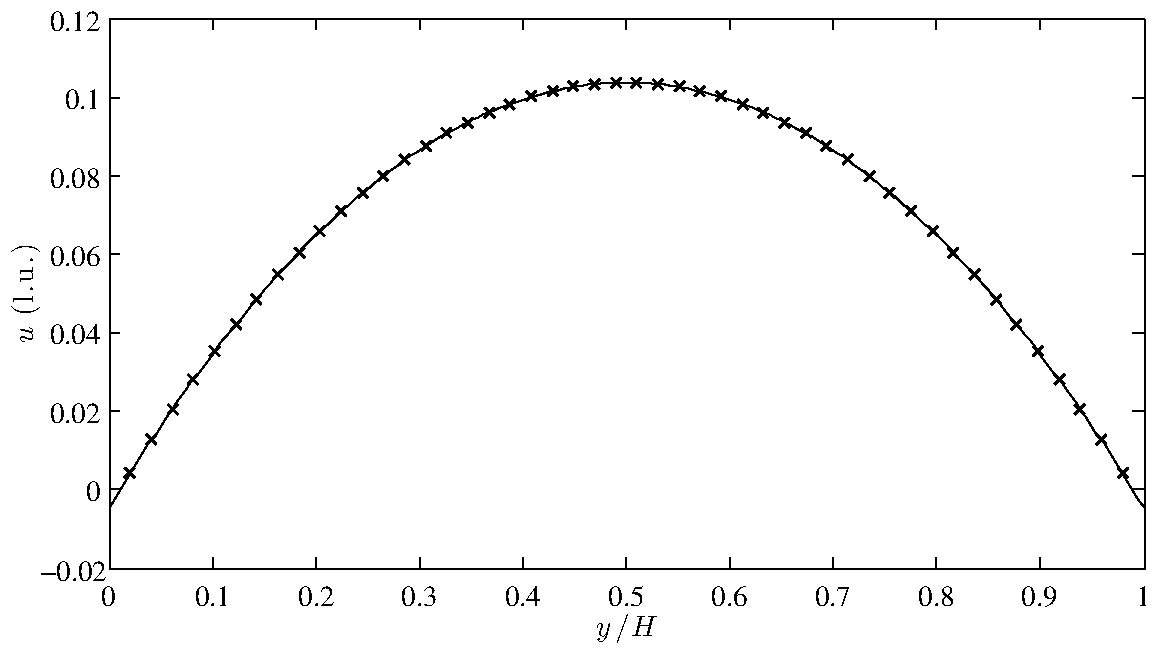
\includegraphics[width=0.9\textwidth]{fig/poiseuille.pdf}
\end{center}
\caption{Obtained velocity profiles of Poiseuille flow ($\times$)
  compared to the analytical solution (solid line). A grid of
  3$\times$50 nodes were used. As expected, there was no variation of
  the velocity field in the flow direction. The velocity is given in
  lattice units.}
\label{fig:mb:poi}
\end{figure}



\section{Taylor-Green vortex}
A more sophisticated system than the Poisseuille flow is the decaying
Taylor-Green vortex flow. Also this system is one of the few where an
analytical solution to the Navier-Stokes equation is possible to
find. In this section, the Taylor-Green flow is used to benchmark the
2D LBM proposed in section \ref{sec:lbm:ns}. A 2D test of the force
implementation is also carried out in section \ref{sec:mb:four_rows}.

The Taylor-Green vortex flow in two dimensions is defined by the
following pressure and velocity fields \cite{junk-asym}:

\begin{equation}\label{eq:mb:tv}
\begin{aligned}
u_x(\x, t) &= -\frac{1}{a}\cos(ax)\sin(by)\exp(-\nu(a^2 +
b^2)t)\\ 
u_y(\x, t) &= \frac{1}{b}\sin(ax)\cos(by)\exp(-\nu(a^2 +
b^2)t)\\ 
P(\x, t) &= -\frac{1}{4} \left( \frac{1}{a^2}\cos(2ax) +
\frac{1}{b^2}\cos(2by)\right) \exp(-2\nu(a^2 + b^2)t)
\end{aligned}
\end{equation}
where $\nu$ is the viscosity, $\x\in[0, 2\pi]^2$ and $a$ and $b$ are
two real constants. It is straight-forward to verify that these
quantities satisfy the incompressible Navier-Stokes,
eqs. \eqref{eq:et:ns_incompressible} and \eqref{eq:et:ns_mom}. The
constants $a$ and $b$ are chosen as $a = b = 2\pi/N$ where $N = N_x =
N_y = 100$ is the grid resolution. This particular choice of $a$ and
$b$ allows us to use lattice units with $\delta_x = \delta_t = 1$ in
the simulation. The maximum velocity in the vortex at $t = 0$ is chosen
as $u_0 = 1/a = 1/b$.

The simulation is performed with $\nu = 0.05$ l.u. on a $100\times100$
lattice. Following the initialisation with the analytical solution,
eq. \eqref{eq:mb:tv}, at $t = 0$, the decay is studied and compared
with the analytical solution. Initialisation of the velocities is done
by setting $\fii = \feq(\rho, \ubf)$ where $\rho$ includes both the
constant density (order $\ep^0$) and the pressure (order $\ep^2$),
compare eq. \eqref{eq:lbm:ns_mom_index}.

The result is presented in fig. \ref{fig:mb:taylor_vis} where the
velocity field and the magnitude of the velocity field is
visualised. This is at a time, $t_{1/2}$, where the maximum magnitude
of the velocity has decreased to half of the initial value,
i.e. $t_{1/2} = \log(2)/(2\nu(2\pi/N)^2)$. In
fig. \ref{fig:mb:taylor_vis}, the analytical and the computed
solutions is compared on a section of the domain at $t = t_{1/2}$. The
agreement with an average error in the order of $10^{-3}$ is
comparable with previous works, e.g. \cite{junk-asym}.


\begin{figure}
  \centering
  \subfloat[Velocity field
    ]{\label{fig:mb:t1}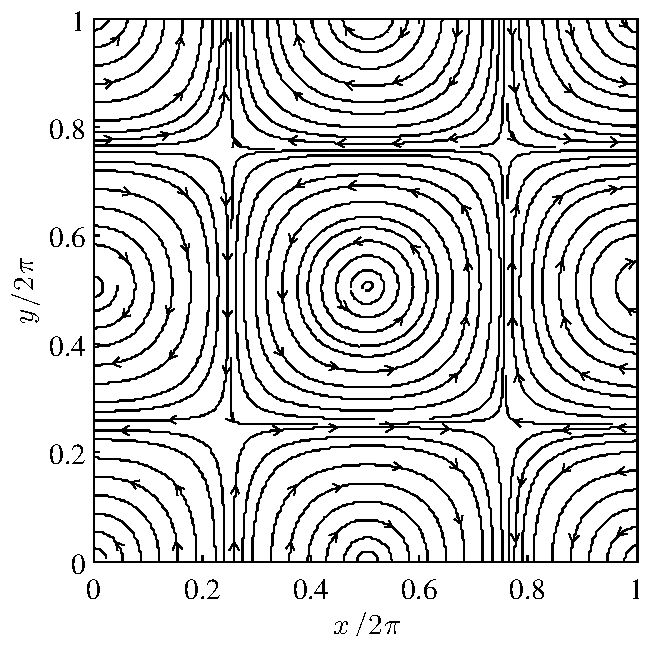
\includegraphics[width=0.47\textwidth]{fig/tg_vortex.pdf}}      
  \hspace{5pt} \subfloat[$|\ubf|$
  ]{\label{fig:mb:t2}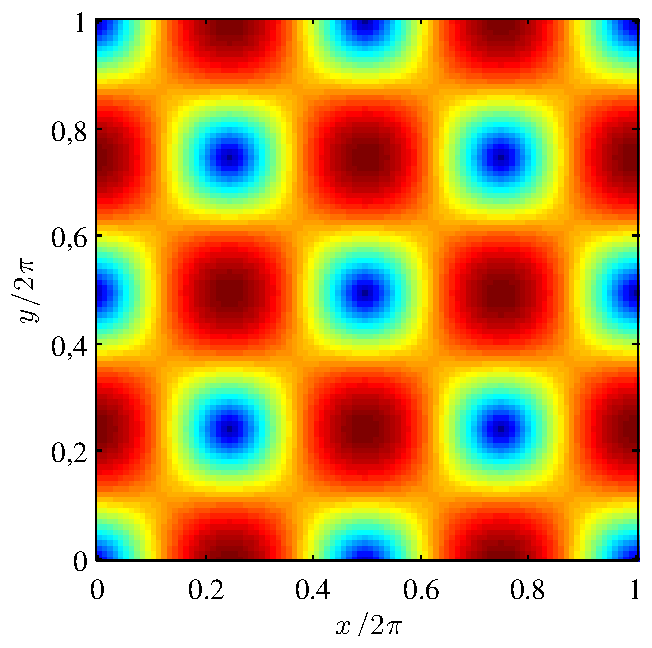
\includegraphics[width=0.47\textwidth]{fig/tg_u.pdf}}
  \caption{Visualised velocity field (a) and magnitude of the
    velocities (b) for a decaying Taylor-Green vortex. The velocity
    field is taken at $t=t_{1/2}$ and the values in (b) varies from
    $-u_0/2$ (blue) to $u_0/2$ (red).}
  \label{fig:mb:taylor_vis}
\end{figure}

\begin{figure}
\begin{center}
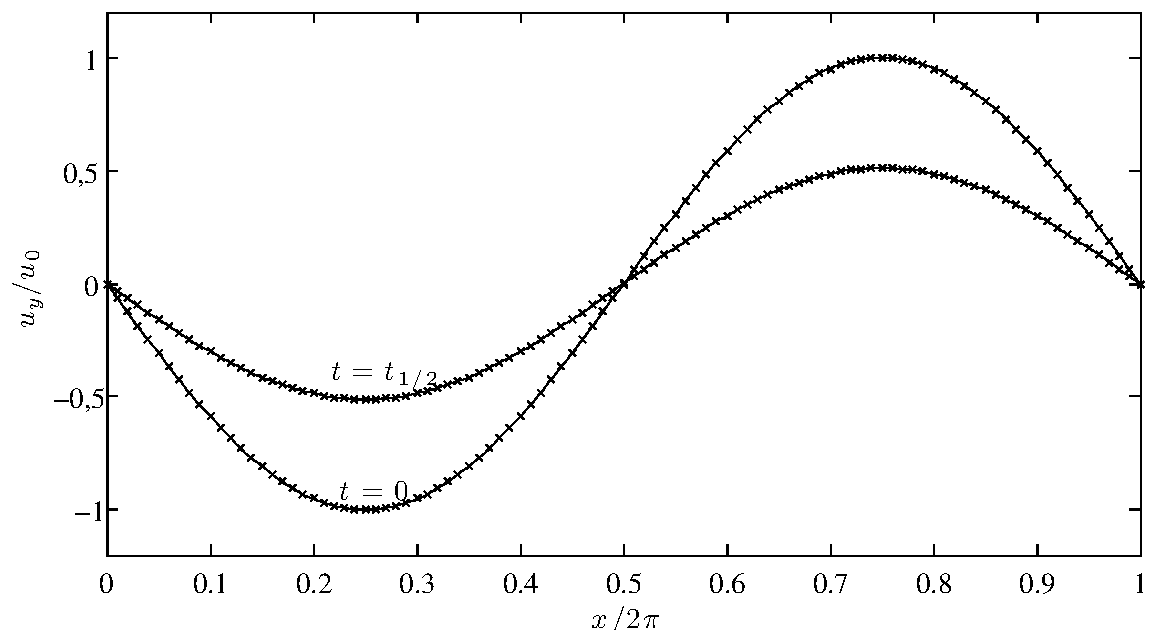
\includegraphics[width=0.9\textwidth]{fig/taylor_uy.pdf}
\end{center}
\caption{1D section of the decaying Taylor-Green flow. The $y$
  component of the velocity is plotted at $y = \pi$. Computed solutions
  ($\times$) are compared with analytical (solid) at two different
  times $t = 0$ and $t = t_{1/2}$. A domain of $100\times100$ nodes
  were used.}
\label{fig:mb:tg_uy}
\end{figure}

\subsection{Four rows mill}\label{sec:mb:four_rows}
In the decaying Taylor-Green flow, the time derivative term in
Navier-Stokes momentum equation is balanced by the viscous term. We
now wish to compensate for the decay by introducing a force. In a
steady state situation: $\partial_t\ubf = 0$ and the force must
balance the viscous term. The force is therefore chosen as

\begin{equation}
\begin{aligned}
F_x(\x, t) &= \nu(a^2 + b^2)u_x(\x, t) \\
F_y(\x, t) &= \nu(a^2 + b^2)u_y(\x, t) 
\end{aligned}
\end{equation}
where $u_x$ and $u_y$ are the velocities from
eq. \eqref{eq:mb:tv}. Using the same parameters, initialisation and
domain as in the decaying case, no decay is observed. In
fig. \ref{fig:mb:four_mill}, a section of the $y$ component of the
velocity is shown at $t = t_{1/2}$.

\begin{figure}
\begin{center}
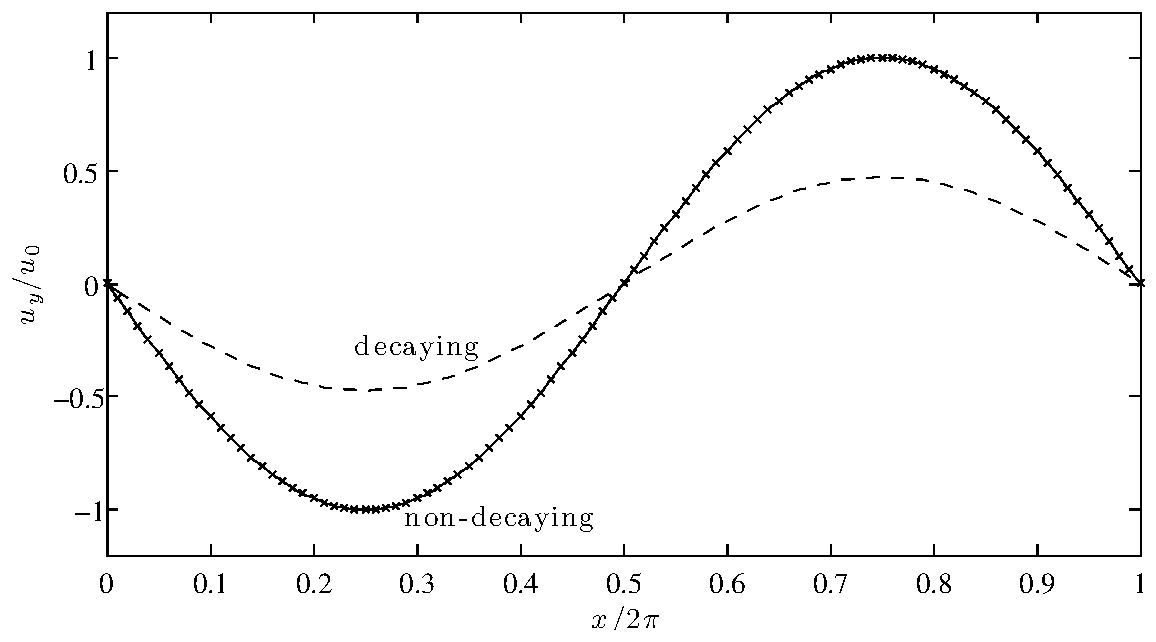
\includegraphics[width=0.9\textwidth]{fig/four_mill.pdf}
\end{center}
\caption{1D section of the steady four rows mills flow at $t =
  t_{1/2}$. An external force have been included to compensate the
  decay (dashed). The $y$ component is plotted for $y = \pi$. We
  observe no decay as the computed solution ($\times$) and the initial
  velocity (solid) coincide.}
\label{fig:mb:four_mill}
\end{figure}



\section{Helmholtz equation}
The LB formulation for solving Poisson's equation as well as the
implementation was tested by solving Helmholtz equation with a
certain set of boundary conditions allowing for finding an analytical
solution. The homogeneous Helmholtz equation reads:

\begin{equation}\label{eq:mb:helmholtz}
\nabla \psirm = \lambda^2 \psirm
\end{equation}
where $\lambda$ is a real parameter. The equation was solved for
$\lambda = 2$ on the domain $(x, y)\in[0, 1]\times[0, 1]$ with the
following Dirichlet boundary conditions:

\begin{equation}\label{eq:mb:helm_bdry}
  \begin{array}{l l}
\psirm(0, y) = -\psirm(1, y) = \frac{\sinh\sqrt{\lambda^2 + \pi^2}(1 -
  y)}{\sinh\sqrt{\lambda^2 + \pi^2}},\\ \psirm(x, 0) =
\cos\pi x,\;\; \psirm(x, 1) = 0.
\end{array}
\end{equation}
The analytical solution to eq. \eqref{eq:mb:helmholtz} with the given
boundary conditions is \cite{chai_poi}:

\begin{equation}
\psirm(x, y) = cos\pi x \frac{\sinh\sqrt{\lambda^2 + \pi^2}(1 -
  y)}{\sinh\sqrt{\lambda^2 + \pi^2}}.
\end{equation}

A grid of $n_x\times n_y = 65\times65$ nodes was used when computing the LBM
solution. The computational domain was rescaled to the desired one by
setting $\delta_x = 1/(n_x-1) = 1/64$ and $\delta_t = \delta_x^2$. An
other possibility would have been to rescale the parameter $\lambda$
and have $\delta_x = \delta_t = 1$.

The boundary conditions in eq. \eqref{eq_mb_helm_bdry} was implemented
using the He/Zou approach described in section \ref{sce:lbm:hezou}. A
bounce back approach with some momentum addition would also have been
possible but was not chosen due to that the actual boundary location
is not at the node location, but half a node-node distance into the
computational domain. Also the bounce-back implementation is
previously tested. 

In fig. \ref{fig:mb:h1}, the obtained solution is presented together
with the absolute error in fig. \ref{fig:mb:h2}. The agreement is
satisfying, with an error which magnitude is about the same as in
previous works \cite{chai_poi}. The error takes on its maximum at the
boundary of the domain, implying that the fulfilment of the boundary
conditions is not complete.



\section{Advection-Diffusion}
Before the implementation of the Nernst-Planck part of the model is
tested, a special case is considered, i.e. when the electrical
potential in the domain is constant. This makes the source term
including the electrical potential in eq. \eqref{nernst-planck} vanish
and we have to solve only for advection and diffusion.

Introducing characteristic scales for the concentration ($C_0$),
advective velocity ($u_0$) and length ($l_0$) respectively, gives the
non-dimensional advection-diffusion equation for incompressible flow:

\begin{equation}\label{non_dim_adv-dif}
\frac{\partial C}{\partial t} + \mathbf{u} \cdot \nabla C = 
\frac{D}{u_0 l_0} \nabla^2C.
\end{equation}

All variables in \eqref{non_dim_adv-dif} are non-dimensional. The
quantity $Pe = u_0l_0/D$ is often referred to as the P\'{e}clet number. It
determines the relation between contributions to the
dynamics from advection and diffusion respectively. For $Pe \gg 1$ the
dynamics is dominated by advection and for $Pe \ll 1$ by diffusion. 

The LB model described in section \ref{sec:nernst-planck_lb} was
tested by studying the evolution in time and space of a point mass in
one dimension. The analytical solution of eq. \eqref{non_dim_adv-dif}
in one dimension with initial conditions $C(x, t = 0) = \delta(x)$ on
an infinite domain is:

\begin{equation}
C(x, t) = \sqrt{\frac{Pe}{4 \pi t}}\exp\left({-\frac{(x - ut)^2
    Pe}{4t}}\right).
\end{equation}

In the numerical computations the parameters $Pe = 10$ and
$|\mathbf{u}| = 0.1$ were used. The domain consisted of 200 lattice
nodes and three snapshots in time at $t = 100, 200, 300$ were compared
to the analytical solution. The result is presented in
fig. \ref{fig:adv-dif}.

\begin{figure}
\begin{center}
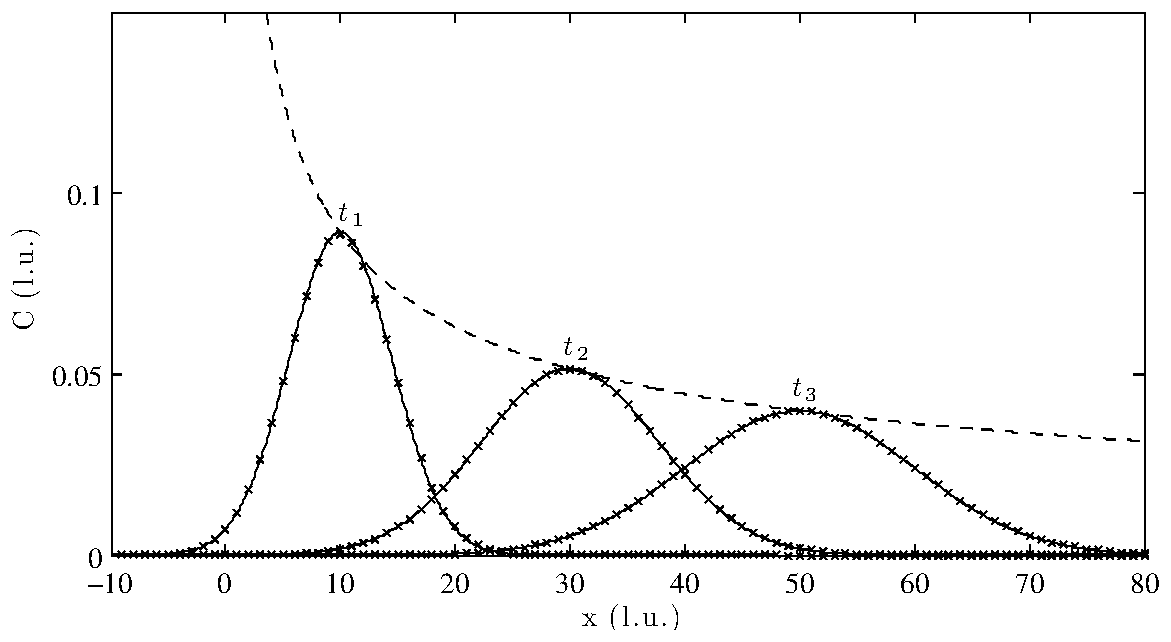
\includegraphics[width=0.9\textwidth]{fig/adv_dif_10_30_50.pdf}
\end{center}
\caption{Obtained solutions ($\times$) of the
  advection-diffusion equation for a point mass evolving in time and
  space. Three different times ($t_n = 100n$) are compared to
  analytical solutions (solid). The Amplitude of the solutions as
  function of time has also been plotted (dashed). The advecting
  velocity, $u_0 = 0.1$ and the Peclet number, $Pe = 10$.  All units
  are in lattice units.}
\label{fig:adv-dif}
\end{figure}


\section{Nernst-Planck, a special case}
This benchmark aims to test the advection due to present electrical
fields in the advection diffusion solver. It is done by solving for
the ion concentration in a system that fulfils the assumptions for the
Poisson-Boltzmann distribution. Beside a system in steady state, the
assumptions are a simple geometry that allows for the one dimensional
integration and a zero advective velocity, see section
\ref{sec:et:pb}. 

A 1:1 ion solution will be considered and therefore two solvers for
the Nernst-Planck equation are needed. One for positive and one for
negative ions. These will be coupled to a solver for Poisson's
equation which will update the potential each time step according to
the present ion concentration. In the steady state, the ion
concentrations for positive and negative ions respectively are
compared to the exponential expression in the Poisson-Boltzmann
situation, eq. \eqref{eq:C}. The potential in this expression is
obtained by solving the Poisson-Boltzmann equation,
eq. \eqref{eq:pb_real}.


Two solvers using the method in section, \ref{sec:lbm:np} are set up
with the following set of parameters:

\begin{itemize}
\item[] z = $\pm$ 1
\item[] D = $10^{-8}$ m$^2$s$^{-1}$
\item[] T = 293 K
\item[] $\epsilon_r$ = 80
\end{itemize}
The Nernst-Planck equation is put on non-dimensional form by
introducing the following characteristic quantities:

\begin{itemize}
\item[] $\cnil$ = $10^{-4}$ mol/m$^3$
\item[] $\lnil$ = 2$\cdot10^{-5}$/ny m
\item[] $\Vnil$ = -50 mV
\item[] $\unil$ = 0.1 m/s.
\end{itemize}
These parameters gives a Peclet number of $\Pe = 2$ which gives a
relaxation parameter $\omega_{NP} = 0.5$.

The geometry of the system simulated is an infinite channel with
straight walls. A grid of 3$\times$100 nodes is used for the
computation, i.e. 100 nodes across the channel. At the walls, the no
flux boundary condition, eq. \eqref{eq:et:j0}, is implied through the
mirror reflection approach described in section,
\ref{sec:lbm:mirror}. For the Poisson solver, a constant surface
charge density of $\sigma = -0.17$ $\mu$C/m$^2$ is applied to the
walls, eq. \eqref{eq:et:fix_c}. This is realised by a modified mirror
reflection, see section \ref{sec:lbm:mod_mirror}.

The charge concentration at the middle of the channel (denoted by
$\C^{\infty}$ in eq. \eqref{eq:C}) in the Poisson-Boltzmann distribution
are set to the values obtained from the Nernst-Planck solver. 

In fig. \ref{fig:mb:np}, the resulting charge distributions are
presented.  

\begin{figure}
\begin{center}
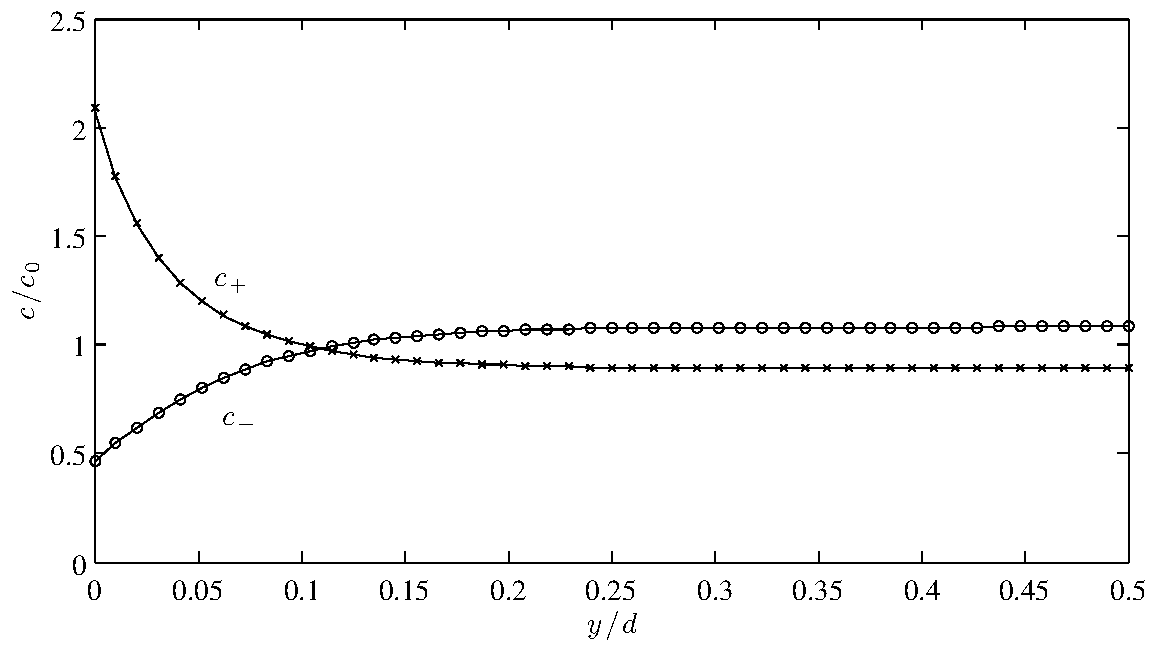
\includegraphics[width=0.9\textwidth]{fig/np_bench.pdf}
\end{center}
\caption[Comparison between the Nernst-Planck and Poisson-Boltzmann
    models.]{Computed charge concentrations for positive ($\C_+$) and
    negative ($\C_{-}$) ions respectively in contact with a negatively
    charged wall. The concentrations are compared with the
    Poisson-Boltzmann distribution (solid).}
\label{fig:mb:np}
\end{figure}





\chapter{Modelling of electrokinetic flow}
kcl ref to appendix...
\begin{table}
  \caption{Physical parameters of a KCl ion solution that is modelled
    in this chapter. Parameters are from \cite{dongquing-ren-book}. }
\begin{center}
    \begin{tabular}{ | r | l |}
    \hline
    Relative permittivity, $\ep_r$ & 80\\
    Mean ionic conentration, $\cnil$ & $10^{-4}$ mol/m$^3$\\
    Conductivity, $\sigma_c$ & 1.5 mS/m\\
    Temperature, T & 293 K\\
    kinematic viscosity, $\nu$ & 1.0 $\mu$m$^2$/s\\
    Diffusion coefficient, $D_+ = D_{-}$ & $ 10^{-10}$ m$^2$/s\\
    \hline
    \end{tabular}
\end{center}    
\label{tab:res:param}
\end{table}

\section{Charge concentration and potential in 1D system}
section in the channel, + debye-huckel comparision

\begin{figure}
\begin{center}
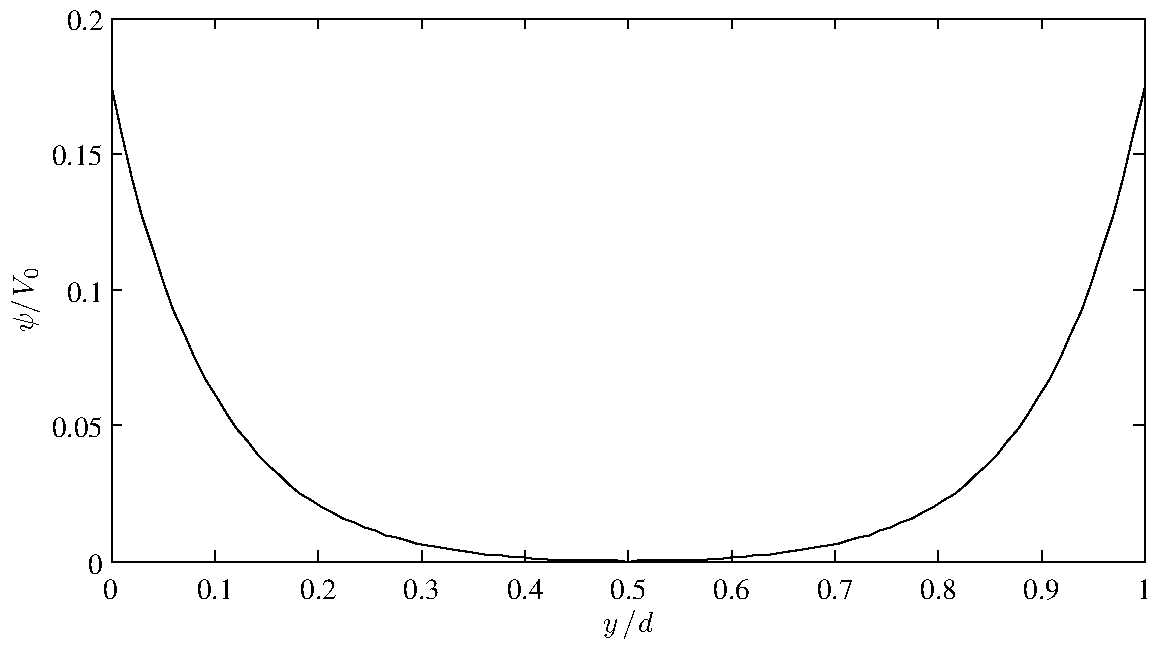
\includegraphics[width=0.9\textwidth]{fig/potential_1d.pdf}
\end{center}
\caption{Computed electric potential across a channel of width $d = 10
  \mu$m. The solution in the channel is a KCl solution defined by
  parameters in table \ref{tab:res:param}. The channel walls are
  negatively charged. Note that $\Vnil$ is negative.}
\label{fig:res:pot_1d}
\end{figure}

\begin{figure}
\begin{center}
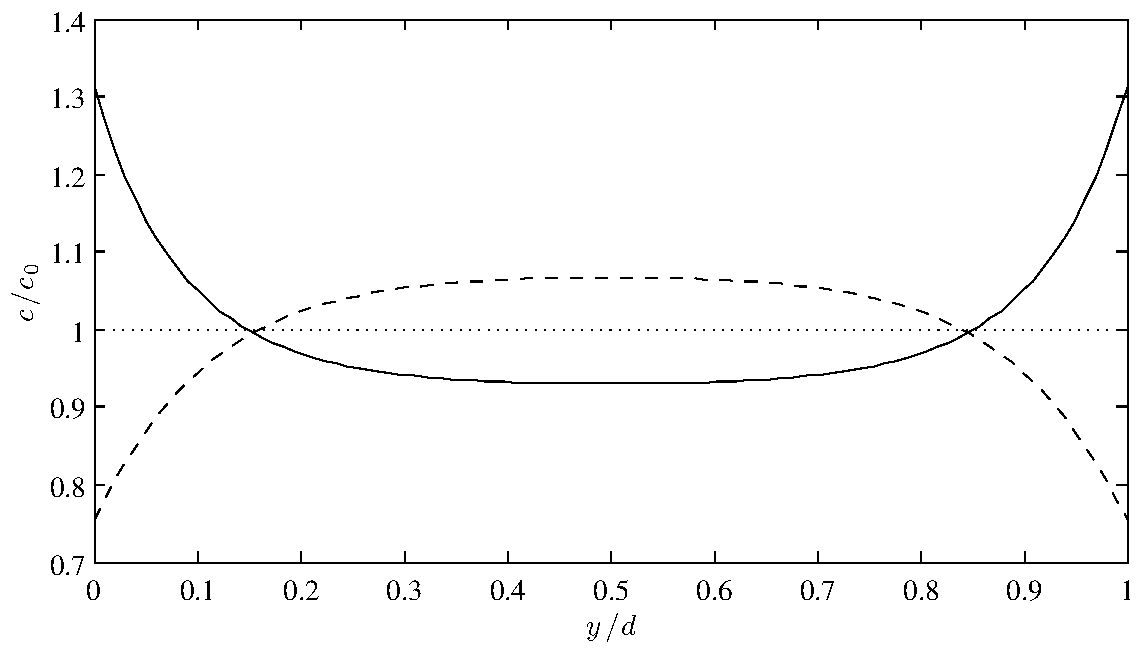
\includegraphics[width=0.9\textwidth]{fig/charge_1d.pdf}
\end{center}
\caption{Computed positive (solid) and negative (dashed) charge
  distribution across a channel of width $d = 10 \mu$m. The solution
  in the channel is a KCl solution defined by parameters in table
  \ref{tab:res:param}. The channel walls are negatively charged.}
\label{fig:res:c_1d}
\end{figure}

\subsection{Nernst-Planck vs. Poisson-Boltzmann}

\section{Electroviscous effect}

\section{Electroosmotic flow}
NP + PB differences?
\section{Flow in channel with heterogeneously charged walls}

\section{Flow in array of charged squares}


\chapter{Conclusions}
And what do we conclude of this?


\newpage
\clearpage

\bibliography{references} % references.bib
\addcontentsline{toc}{chapter}{\numberline{} Bibliography} % For pdf
%\setspecialhdr

\newpage

% Appendices
\appendix
\setdefaulthdr
\chapter{Code snippet}\label{app:poi_snippet}
An example code defining Poiseuille flow driven by a constant force
(pressure gradient) using the LBM library developed in this work.
\begin{verbatim}
#include <iostream>
#include "../LBM.h"

using namespace std;

int main(){
  int nx = 3, ny = 50, tMax = 1000;
  double w = 0.75;
  double c = 1.0;

  LatticeModel *lm = new Lattice2D(nx, ny);
  StreamD2Q9Periodic *sm = new StreamD2Q9Periodic();
  CollisionD2Q9BGKNSF *cm = new CollisionD2Q9BGKNSF();
  LBM *lbm = new LBM(lm, cm, sm);

  double **fx = allocate2DArray(ny, nx);
  double **fy = allocate2DArray(ny, nx);

  cm->setW(w);
  cm->setC(c);


  /* Set boundary conditions*/
  BounceBackNodes<CollisionD2Q9BGKNSF> *bbns =
          new BounceBackNodes<CollisionD2Q9BGKNSF>();
  bbns->setCollisionModel(cm);
  for(int i = 0; i < nx; i++){
    bbns->addNode(i, 0, 0);
    bbns->addNode(i, ny-1, 0);
  }
  lbm->addBoundaryNodes(bbns);

  /* Set force */
  for(int i = 0; i < nx; i++){
    for(int j = 0; j < ny; j++){
      fx[j][i] = 0.0001;
      fy[j][i] = 0.0;
    }
  }
  cm->setForce(fx, fy);

  /* Initialize solver */
  lbm->init();

  /* Main loop */
  for(int t = 0; t < tMax; t++){
    lbm->collideAndStream();
  }

  cm->dataToFile("bench_force_poi/");

  return 0;
}
\end{verbatim}

\end{document}
